% Options for packages loaded elsewhere
\PassOptionsToPackage{unicode}{hyperref}
\PassOptionsToPackage{hyphens}{url}
%
\documentclass[
]{book}
\usepackage{amsmath,amssymb}
\usepackage{lmodern}
\usepackage{ifxetex,ifluatex}
\ifnum 0\ifxetex 1\fi\ifluatex 1\fi=0 % if pdftex
  \usepackage[T1]{fontenc}
  \usepackage[utf8]{inputenc}
  \usepackage{textcomp} % provide euro and other symbols
\else % if luatex or xetex
  \usepackage{unicode-math}
  \defaultfontfeatures{Scale=MatchLowercase}
  \defaultfontfeatures[\rmfamily]{Ligatures=TeX,Scale=1}
\fi
% Use upquote if available, for straight quotes in verbatim environments
\IfFileExists{upquote.sty}{\usepackage{upquote}}{}
\IfFileExists{microtype.sty}{% use microtype if available
  \usepackage[]{microtype}
  \UseMicrotypeSet[protrusion]{basicmath} % disable protrusion for tt fonts
}{}
\makeatletter
\@ifundefined{KOMAClassName}{% if non-KOMA class
  \IfFileExists{parskip.sty}{%
    \usepackage{parskip}
  }{% else
    \setlength{\parindent}{0pt}
    \setlength{\parskip}{6pt plus 2pt minus 1pt}}
}{% if KOMA class
  \KOMAoptions{parskip=half}}
\makeatother
\usepackage{xcolor}
\IfFileExists{xurl.sty}{\usepackage{xurl}}{} % add URL line breaks if available
\IfFileExists{bookmark.sty}{\usepackage{bookmark}}{\usepackage{hyperref}}
\hypersetup{
  pdftitle={What makes an R-package popular?},
  pdfauthor={Yiwen Zhang},
  hidelinks,
  pdfcreator={LaTeX via pandoc}}
\urlstyle{same} % disable monospaced font for URLs
\usepackage{longtable,booktabs,array}
\usepackage{calc} % for calculating minipage widths
% Correct order of tables after \paragraph or \subparagraph
\usepackage{etoolbox}
\makeatletter
\patchcmd\longtable{\par}{\if@noskipsec\mbox{}\fi\par}{}{}
\makeatother
% Allow footnotes in longtable head/foot
\IfFileExists{footnotehyper.sty}{\usepackage{footnotehyper}}{\usepackage{footnote}}
\makesavenoteenv{longtable}
\usepackage{graphicx}
\makeatletter
\def\maxwidth{\ifdim\Gin@nat@width>\linewidth\linewidth\else\Gin@nat@width\fi}
\def\maxheight{\ifdim\Gin@nat@height>\textheight\textheight\else\Gin@nat@height\fi}
\makeatother
% Scale images if necessary, so that they will not overflow the page
% margins by default, and it is still possible to overwrite the defaults
% using explicit options in \includegraphics[width, height, ...]{}
\setkeys{Gin}{width=\maxwidth,height=\maxheight,keepaspectratio}
% Set default figure placement to htbp
\makeatletter
\def\fps@figure{htbp}
\makeatother
\setlength{\emergencystretch}{3em} % prevent overfull lines
\providecommand{\tightlist}{%
  \setlength{\itemsep}{0pt}\setlength{\parskip}{0pt}}
\setcounter{secnumdepth}{5}
\usepackage{booktabs}
\usepackage{amsthm}
\usepackage{bera}
\usepackage{tcolorbox}
\makeatletter
\def\thm@space@setup{%
  \thm@preskip=8pt plus 2pt minus 4pt
  \thm@postskip=\thm@preskip
}
\makeatother

\newenvironment{discovery}[1]{%
  \begin{tcolorbox}[colback=blue!30,colframe=blue!80!black]#1}{\end{tcolorbox}}
\usepackage{booktabs}
\usepackage{longtable}
\usepackage{array}
\usepackage{multirow}
\usepackage{wrapfig}
\usepackage{float}
\usepackage{colortbl}
\usepackage{pdflscape}
\usepackage{tabu}
\usepackage{threeparttable}
\usepackage{threeparttablex}
\usepackage[normalem]{ulem}
\usepackage{makecell}
\usepackage{xcolor}
\ifluatex
  \usepackage{selnolig}  % disable illegal ligatures
\fi
\usepackage[style=authoryear,]{biblatex}
\addbibresource{book.bib}
\addbibresource{packages.bib}

\title{What makes an R-package popular?}
\author{Yiwen Zhang}
\date{2021-06-11}

\begin{document}
\maketitle

{
\setcounter{tocdepth}{1}
\tableofcontents
}
\hypertarget{preface}{%
\chapter*{Preface}\label{preface}}
\addcontentsline{toc}{chapter}{Preface}

As an R user, have you ever thought about what kind of information is hidden behind the number of downloads for R and R-packages? Why would there an abnormal download value? When choosing which package to use, we often probably tend to use popular ones. But what kind of packages are popular? And What factors will linked to the popularity of an R-package? I suppose these are questions that most R users will be curious about. Therefore, based on the existing findings, this report answers the above questions to a certain extent by taking an exploratory data analysis.

This is written as part of the ETC5543 research project supervised by Drs Emi Tanaka and Hien Nguyen. Due to the limitations of my programming ability, I encountered some obstacles during this research. But this is also a very precious opportunity for me to cultivate my research thinking and improve my confidence in coding.

I would like to express my very great appreciation to Drs Emi Tanaka and Hien Nguyen for their valuable and constructive suggestions during the planning and development of this research work. As my supervisors, their patient guidance, enthusiastic encouragement and willingness to give their time so generously have been very much appreciated. And my special thanks are also extended to Dr Emi Tanaka for her generous help on writing. I would like to also thank Professor Rob J Hyndman, for holding every two weeks' meeting to give us recommendations.

I hope you enjoy your reading.

\hypertarget{abstract}{%
\chapter{Abstract}\label{abstract}}

This research seeks to analyze the popularity of R-packages and figure out the influential factors. Data are closely related to social and economic activities in our daily life, so data mining and analysis will definitely benefit us. In many statistical and data analysis tools, this research focuses on R in this project, and aim to explore the popularity of R-packages from CRAN. To achieve this, it is assumed in this research that the download volume is a relatively reliable and simple measurement for the popularity of R-packages, and two main parts of analysis has been carried out, one is to uncover the information behind the download count logs, the other is to explore the factors that will linked to the download volume. The techniques applied in this research is mainly R, together with a small part of Python on data scraping. By obtaining the daily and recent half a year's total download count of 17,699 R-packages and R itself, this research analyzes their pattern characteristics, as well as the relationship between the release date, update times, number of commits on Github, name length and alphabetic order of the name. Finally, this research also gives the changes of R-user preferences on 1st April from 2013 to 2021, to some extent.

Moreover, results show that the daily download of R-packages has a strong weekly seasonality and unusual spikes caused by repeat download, update or server issue. The most stably popular R-packages during 2017 to 2019 is about JAVA dependency. And an earlier release date is more likely to bring a higher download volume for R-packages. That is similar to update times and commits number on Github repository. However, the alphabetical order of R-package name contributes little to the download counts. And over half of the R-packages on CRAN tend to have shorter names.

KEY WORDS : R-package popularity, CRAN download count, Web scraping, Github API, EDA

\hypertarget{intro}{%
\chapter{Introduction}\label{intro}}

Data, which has penetrated into every industry and business field, has become an increasingly important production factor and consumption in our lives. However, data itself must be processed to uncover the information within it. For this reason many statistical tools were born, such as SPSS, Python, R and so on. In this project, we focus on the R language \autocite{R-base}.

R is a language and environment for statistical computing and graphics which can be extended easily via packages and provide an Open Source route to participation in statistical methodology. It is available as Free Software under the term of the Free Software Foundation's GNU General Public License \autocite{gnu}. R is one of the most popular statistical languages and has been ranking competitively even among the general purpose programming languages \autocite[peaking 8th in August 2020 in][]{tiobe}. The TIOBE Programming Community index aggregates several search engines to derive a metric of the popularity of a programming language. It is important to note, however, that programming languages ranked higher than R are mostly general purpose languages and therefore naturally has a larger user base whereas R is exclusively for data analysis and statistical computation alone.

Today, R is greatly enhanced by over 17,699 R-packages contributed by hundreds of developers all over the world. However, when R originally appeared in August of 1993 with its first official release in June of 1995 \autocite{Ikaha1998}, the contributions were managed by only a small group of core developers. In April of 1997, Comprehensive R Archive Network (CRAN) was established as the official R-packages repository with 3 mirror sites. Now the source repositories to install R-packages have expanded to Bioconductor, Gitlab, GitHub, R-Forge and \href{https://cran.r-project.org/mirmon_report.html}{106 CRAN mirrors in 49 regions}. Of all the CRAN mirrors, the daily download count for each package is only readily available from the RStudio CRAN mirror. In this report, we will be focusing only on one CRAN mirror via RStudio, albeit the most popular one, for exploratory data analysis. Henceforth, all download counts of packages refer to the download from this RStudio CRAN mirror.

CRAN is a network of ftp and web servers around the world that store identical, up-to-date, versions of code and documentation for R \autocite{CRAN}.

The most intuitive embodiment of popularity is the total number of downloads, although it does not directly reflect the number of users, because it includes the repeated downloads by the same user, updates and test downloads caused by the server. Briefly, some works that use these download counts include: the R-package \texttt{adjustedcranlogs} \autocite{adjustedcranlogs} attempts to correct this download inflation using a heuristic approach; package \texttt{packageRank} \autocite{packageRank} provides a way to compute the rank percentile for packages and filter the invalid downloads including small and medium size logs. What's more, there are also some packages such as \texttt{pkgsearch}\autocite{pkgsearch} and \texttt{Visualize.CRAN.Downloads}\autocite{VisualizeCRANDownloads} providing some visualization methods to explore the package download trend or for convenient searching. More details are explained in Section 5.

Based on that, researchers have started to study the popularity of R-packages from CRAN. And we still assume in this project that, the download amount is a relatively reliable and simple measure of packages' popularity. Back to the previous studies, the R-package \texttt{adjustedcranlogs}\autocite{adjustedcranlogs} finds that there are spikes in downloads due to automatic re-downloads and package update, and it also provides a method to remove these download logs. Some of them are function extensions based on previous packages, and some of them propose their own new functions, but generally speaking, they are inclined to be more tool like to help users explore the characteristics of package download logs from as many dimensions as possible.

As for us, the purpose of this project is to explore the download logs of R-packages on CRAN and analyze the relationship between some influential factors with it to help users and developers better understand the download amount pattern, and also figure out what would determine a package's popularity to some extent.

\begin{itemize}
\item
  CRAN mirror is a website containing differently located servers, which aims to facilitate people from different regions and countries to access CRAN more smoothly and quickly. And each server is called a mirror \autocite{cranmirror}.
\item
  CRAN task view : It aims to provide some guidance which packages on CRAN are relevant for tasks related to a certain topic \autocite{crantaskviews}.
\end{itemize}

\hypertarget{other-work}{%
\section{Other work}\label{other-work}}

\texttt{adjustedcranlogs}: More specifically, any unusual download spikes are smoothed over and the upward download bias is removed stochastically by subtracting the minimum download count from a random sampling of packages; if this corrected download results in a negative value then this is adjusted to be zero.

\hypertarget{data}{%
\chapter{Data}\label{data}}

The main source of data used in this report is the download logs from the RStudio CRAN mirror site \url{https://cran.rstudio.com/}. These log files are created for every instance of download of an R-package via the RStudio CRAN mirror, then these log files are processed daily into CSV files that contain the following variables with the name of header in brackets:

\begin{itemize}
\tightlist
\item
  Date (\texttt{date}),
\item
  Time in UTC time zone (\texttt{time}),
\item
  Size of the file in bytes (\texttt{size}),
\item
  Version of R used to download the package (\texttt{r\_version}),
\item
  Architecture type for R (i386 = 32 bit, x86\_64 = 64 bit) (\texttt{r\_arch}),
\item
  Operating System (darwin9.8.0 = mac, mingw32 = windows) (\texttt{r\_os}),
\item
  Package (\texttt{package}),
\item
  Country in two letter ISO country code (\texttt{country}), and
\item
  Anonymised daily unique id (\texttt{ip\_id}).
\end{itemize}

A similar log file is also created for every download of R from the RStudio CRAN mirror with the processed log file generating a CSV file that contains the same variables except \texttt{r\_arch} and \texttt{package}, and \texttt{r\_version} and \texttt{r\_os} are named as \texttt{version} and \texttt{os}. These CSV files are hosted at \url{http://cran-logs.rstudio.com/} and updated daily with data available from 1st October 2012.

The log files of a particular day is processed and compressed into a single CSV file of about 40 megabytes (file sizes of earlier years are much smaller due to lower number of download logs). As there are over 700,000 CSV files, a simple estimate of the size of the data is 28 terabytes - far exceeding typical portable hard drives which are 1-4 terabytes.

The summarised version of data, where the data shows the total daily download count for each package, is accessible using the \texttt{cranlogs} R-package. The \texttt{cranlogs} package accesses this summary data through the web application programming interface (API) maintained by r-hub \autocite{rhub}.

\hypertarget{methods}{%
\chapter{Methods}\label{methods}}

In this project, we extracted R-package names from CRAN and got summary daily download logs of R-packages through web Application Programming Interface (API) maintained by r-hub\autocite{rhub}. And we also collected release dates of R-packages through CRAN. In addition, we also tried to scrap the number of commits in Github repository for R-packages. Then we constructed eight exploratory data analysis sections:

\begin{itemize}
\item
  we explored the daily download of all the packages on CRAN and figured out the number of R-packages occupied by different downloaded groups;
\item
  we analyzed the daily download trend of R itself and the found out the most popular version of R;
\item
  we compared the top 15 downloaded R-packages on CRAN on 1st April. from year 2013 to 2021 to see how the user preference changes;
\item
  we figured out the relationship between initial release date and the total download count for last half a year;
\item
  we compared two closely related packages \texttt{fable} and \texttt{forecast} to see the difference between their MA (moving average);
\item
  we studied how the number of commits of master (main) branch on Github repository may influence the total download count for last half a year;
\item
  we explored the relationship between the number of updates of R-packages and its download count;
\item
  we analyzed the name length pattern for both CRAN task view packages and all the R-packages on CRAN;
\item
  we explored how the alphabetical order of R-packages would related to the download count and its statistic features (variance, median).
\end{itemize}

\hypertarget{results}{%
\chapter{Results}\label{results}}

\hypertarget{daily-download-of-r-packages}{%
\section{Daily download of R-packages}\label{daily-download-of-r-packages}}

\begin{discovery}
\textbf{Finding 1}: There was unusual download activity in one day of
2014 and 2018.
\end{discovery}

In this first section, we studied the daily downloads of CRAN R-packages from 2012-10-01 to 2021-06-07. The data was obtained from the \texttt{cranlogs} package\autocite{cranlogs}, which includes a summary of the download logs from the RStudio CRAN mirror. The daily download data for CRAN R-packages are available from 1st October 2012. Examination of this data showed two unusual observations in 2014 and 2018 as shown in Figure \ref{fig:unusual-spikes}. The one happening in 2014 was on 2014-11-17, which was Monday, while the other one happening in 2018 was on 2018-10-21, which was on Sunday.



\begin{figure}

{\centering 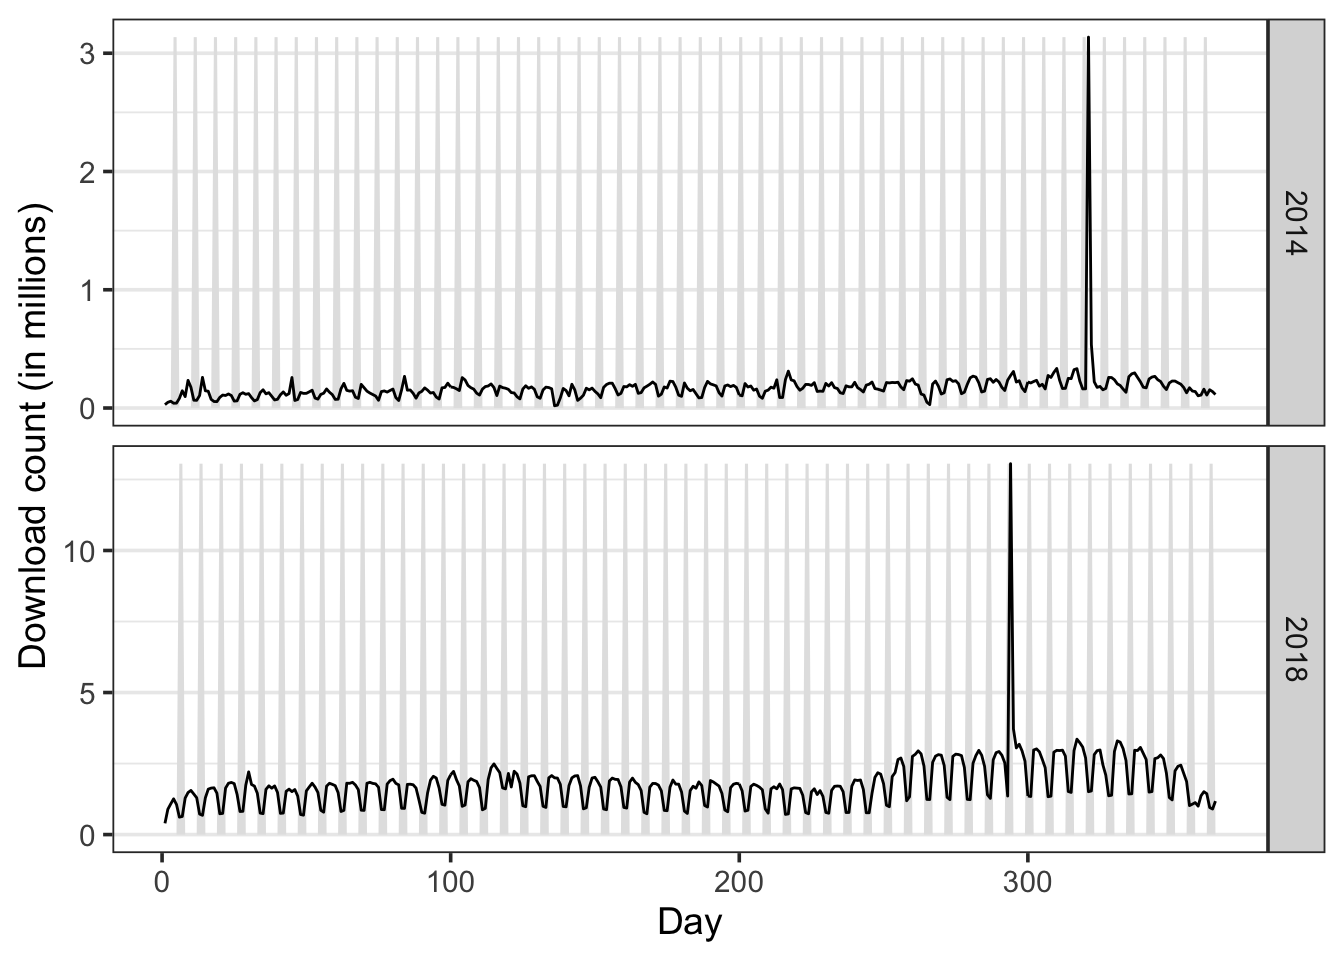
\includegraphics{figures/unusual-spikes-1} 

}

\caption{Unusual download spikes on 2014 and 2018.}\label{fig:unusual-spikes}
\end{figure}

Then let's have a closer look into these two spikes. First, we focused on the spike on 2014-11-17. From Table \ref{tab:spike14count}, we could see that the downloads of top downloaded R-packages on this day differs little, so it's not due to certain package.

\begin{table}

\caption{\label{tab:spike14count}The total downloads of each R-package on 2014-11-17}
\centering
\begin{tabular}[t]{l|r}
\hline
package & n\\
\hline
BayHaz & 767035\\
\hline
clhs & 660298\\
\hline
GPseq & 394840\\
\hline
OPI & 382518\\
\hline
YaleToolkit & 370513\\
\hline
survsim & 224994\\
\hline
BAT & 40592\\
\hline
Rcpp & 3509\\
\hline
ggplot2 & 3167\\
\hline
plyr & 3150\\
\hline
\end{tabular}
\end{table}

Table \ref{tab:spike14country} shows the downloads from different countries. It is obvious that downloads from Indonesia is much more than any others, which indicates the most downloads are from Indonesia.

\begin{table}

\caption{\label{tab:spike14country}The countries downloading from CRAN on 2014-11-17}
\centering
\begin{tabular}[t]{l|r}
\hline
country & n\\
\hline
ID & 2863576\\
\hline
US & 96336\\
\hline
CN & 32729\\
\hline
DE & 14548\\
\hline
FR & 11860\\
\hline
GB & 10491\\
\hline
IN & 8635\\
\hline
HK & 8090\\
\hline
BE & 7720\\
\hline
KR & 6794\\
\hline
\end{tabular}
\end{table}

Furthermore, we also checked the IP address in Table \ref{tab:spike14ip}, downloads from \texttt{ip3758} is much higher than others. So, it seems that most of the downloads are owing to one certain IP.

\begin{table}

\caption{\label{tab:spike14ip}The IP address downloading from CRAN on 2014-11-17}
\centering
\begin{tabular}[t]{r|r}
\hline
ip\_id & n\\
\hline
3758 & 2863432\\
\hline
11536 & 6244\\
\hline
11725 & 5992\\
\hline
16385 & 5991\\
\hline
534 & 5986\\
\hline
3784 & 5983\\
\hline
18519 & 4511\\
\hline
80 & 2124\\
\hline
27 & 1892\\
\hline
464 & 1375\\
\hline
\end{tabular}
\end{table}

Next, let's turn to the one in 2018. Table \ref{tab:spike18count} shows the downloads from tidyverse is much higher than others with nearly three orders of magnitude.

\begin{table}

\caption{\label{tab:spike18count}The total downloads of each R-package on 2014-11-17}
\centering
\begin{tabular}[t]{l|r}
\hline
package & n\\
\hline
tidyverse & 11692582\\
\hline
Rcpp & 16263\\
\hline
stringi & 13981\\
\hline
rlang & 13796\\
\hline
ggplot2 & 13306\\
\hline
dplyr & 13081\\
\hline
glue & 12593\\
\hline
digest & 12302\\
\hline
stringr & 11505\\
\hline
fansi & 11275\\
\hline
\end{tabular}
\end{table}

As for the country, from Table \ref{tab:spike18country} we could know that US is much higher than any other country.

\begin{table}

\caption{\label{tab:spike18country}The countries downloading from CRAN on 2014-11-17}
\centering
\begin{tabular}[t]{l|r}
\hline
country & n\\
\hline
US & 12140853\\
\hline
NA & 179847\\
\hline
GB & 76624\\
\hline
IN & 51502\\
\hline
CN & 46095\\
\hline
TR & 36590\\
\hline
AU & 35078\\
\hline
DE & 32837\\
\hline
CA & 31125\\
\hline
KR & 30469\\
\hline
\end{tabular}
\end{table}

Finally, the most interesting finding is in IP address displayed in Table \ref{tab:spike18ip}. Several consecutive IPs have highly distinguished downloads. It seems that they are from same person, or it is also probably a server test issue in the same short period of time.

\begin{table}

\caption{\label{tab:spike18ip}The IP address downloading from CRAN on 2014-11-17}
\centering
\begin{tabular}[t]{r|r}
\hline
ip\_id & n\\
\hline
266 & 3034720\\
\hline
263 & 2457383\\
\hline
655 & 2099321\\
\hline
264 & 1557640\\
\hline
267 & 1406876\\
\hline
265 & 1032535\\
\hline
2 & 179711\\
\hline
268 & 99932\\
\hline
112 & 34397\\
\hline
3296 & 17223\\
\hline
\end{tabular}
\end{table}

To sum up, we found that these two unusual spikes have one thing in common, that is, most of the downloads came from a specific country. The difference is that in 2014, a large number of downloads came from several different R-packages, while in 2018, they came from only one package \texttt{tidyverse}. In addition, in 2014, a large number of downloads came from one IP, while in 2018, they came from several consecutive IPs, At this point, we guess it should come from the same person, and it is likely to be sever test issue, for it may be not necessary or reasonable for an individual to generate such a large quantities of downloads in one day.

\begin{discovery}
\textbf{Finding 2}: There is an increasing number of downloads over
time. This likely attests to the growing number of R users.
\end{discovery}

Figure \ref{fig:download-over-time} shows the download trend of all R-packages on CRAN over time after fixing the unusual spikes. It shows an upward trend over time, and the variance also increases with the download count, which means the volatility of the data is increasing.



\begin{figure}

{\centering 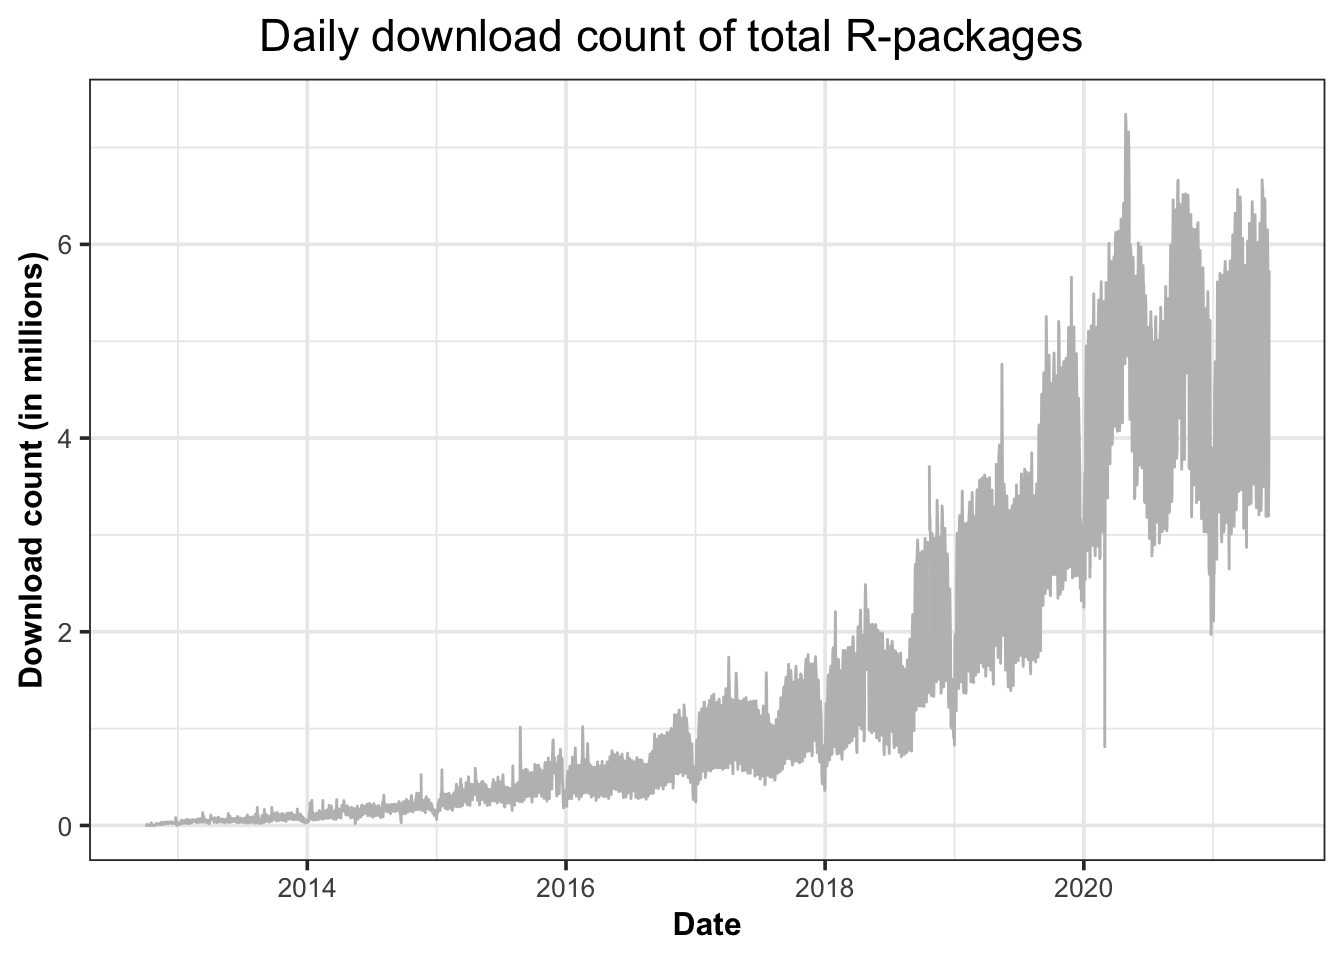
\includegraphics{figures/download-over-time-1} 

}

\caption{The download trend of all R-packages on CRAN over time.}\label{fig:download-over-time}
\end{figure}

\begin{discovery}
\textbf{Finding 3}: Weekends have a lower download than weekdays.
\end{discovery}

To have a closer look at the weekly pattern, figure \ref{fig:total-trend} shows the daily downloads of all CRAN R-packages from the RStudio mirror with the grey areas highlighting the weekend.

To be more specific, we could know that except for 2012 and 2013, the patterns of other years are very similar, that is, they all show strong weekly seasonality. To be more detailed, in 2012, the download logs showed an overall upward trend, because more and more users began to download R-packages from CRAN after its open. In the following years, there is no obvious trend in download volume, but a strong seasonality, which indicates that in a week, the total downloads always increases first then decreases, and reaches the lowest at the weekend. Although the pattern of 2013 is more volatile, it still conforms to that. We think for 2013, that is because CRAN is only open for a short time at this time, and the amount of data downloaded is not adequate to show its download pattern very clearly. Considering this, we could see that after 2016, the pattern of each year is quite consistent, for the total download has been increasing year by year. Back to weekly seasonality, that is because people are more likely to download and use packages in weekdays, and rest on weekends. And that's why the trough of download curve always occurs on weekends. In addition, we could also notice that the lowest downloads across the year are always at the end of December and the beginning of January, probably due to the Christmas and New Year's holidays. What's more, the downloads is on the rise from August to October and from February to April, which covers the start of semester for most universities.



\begin{figure}

{\centering 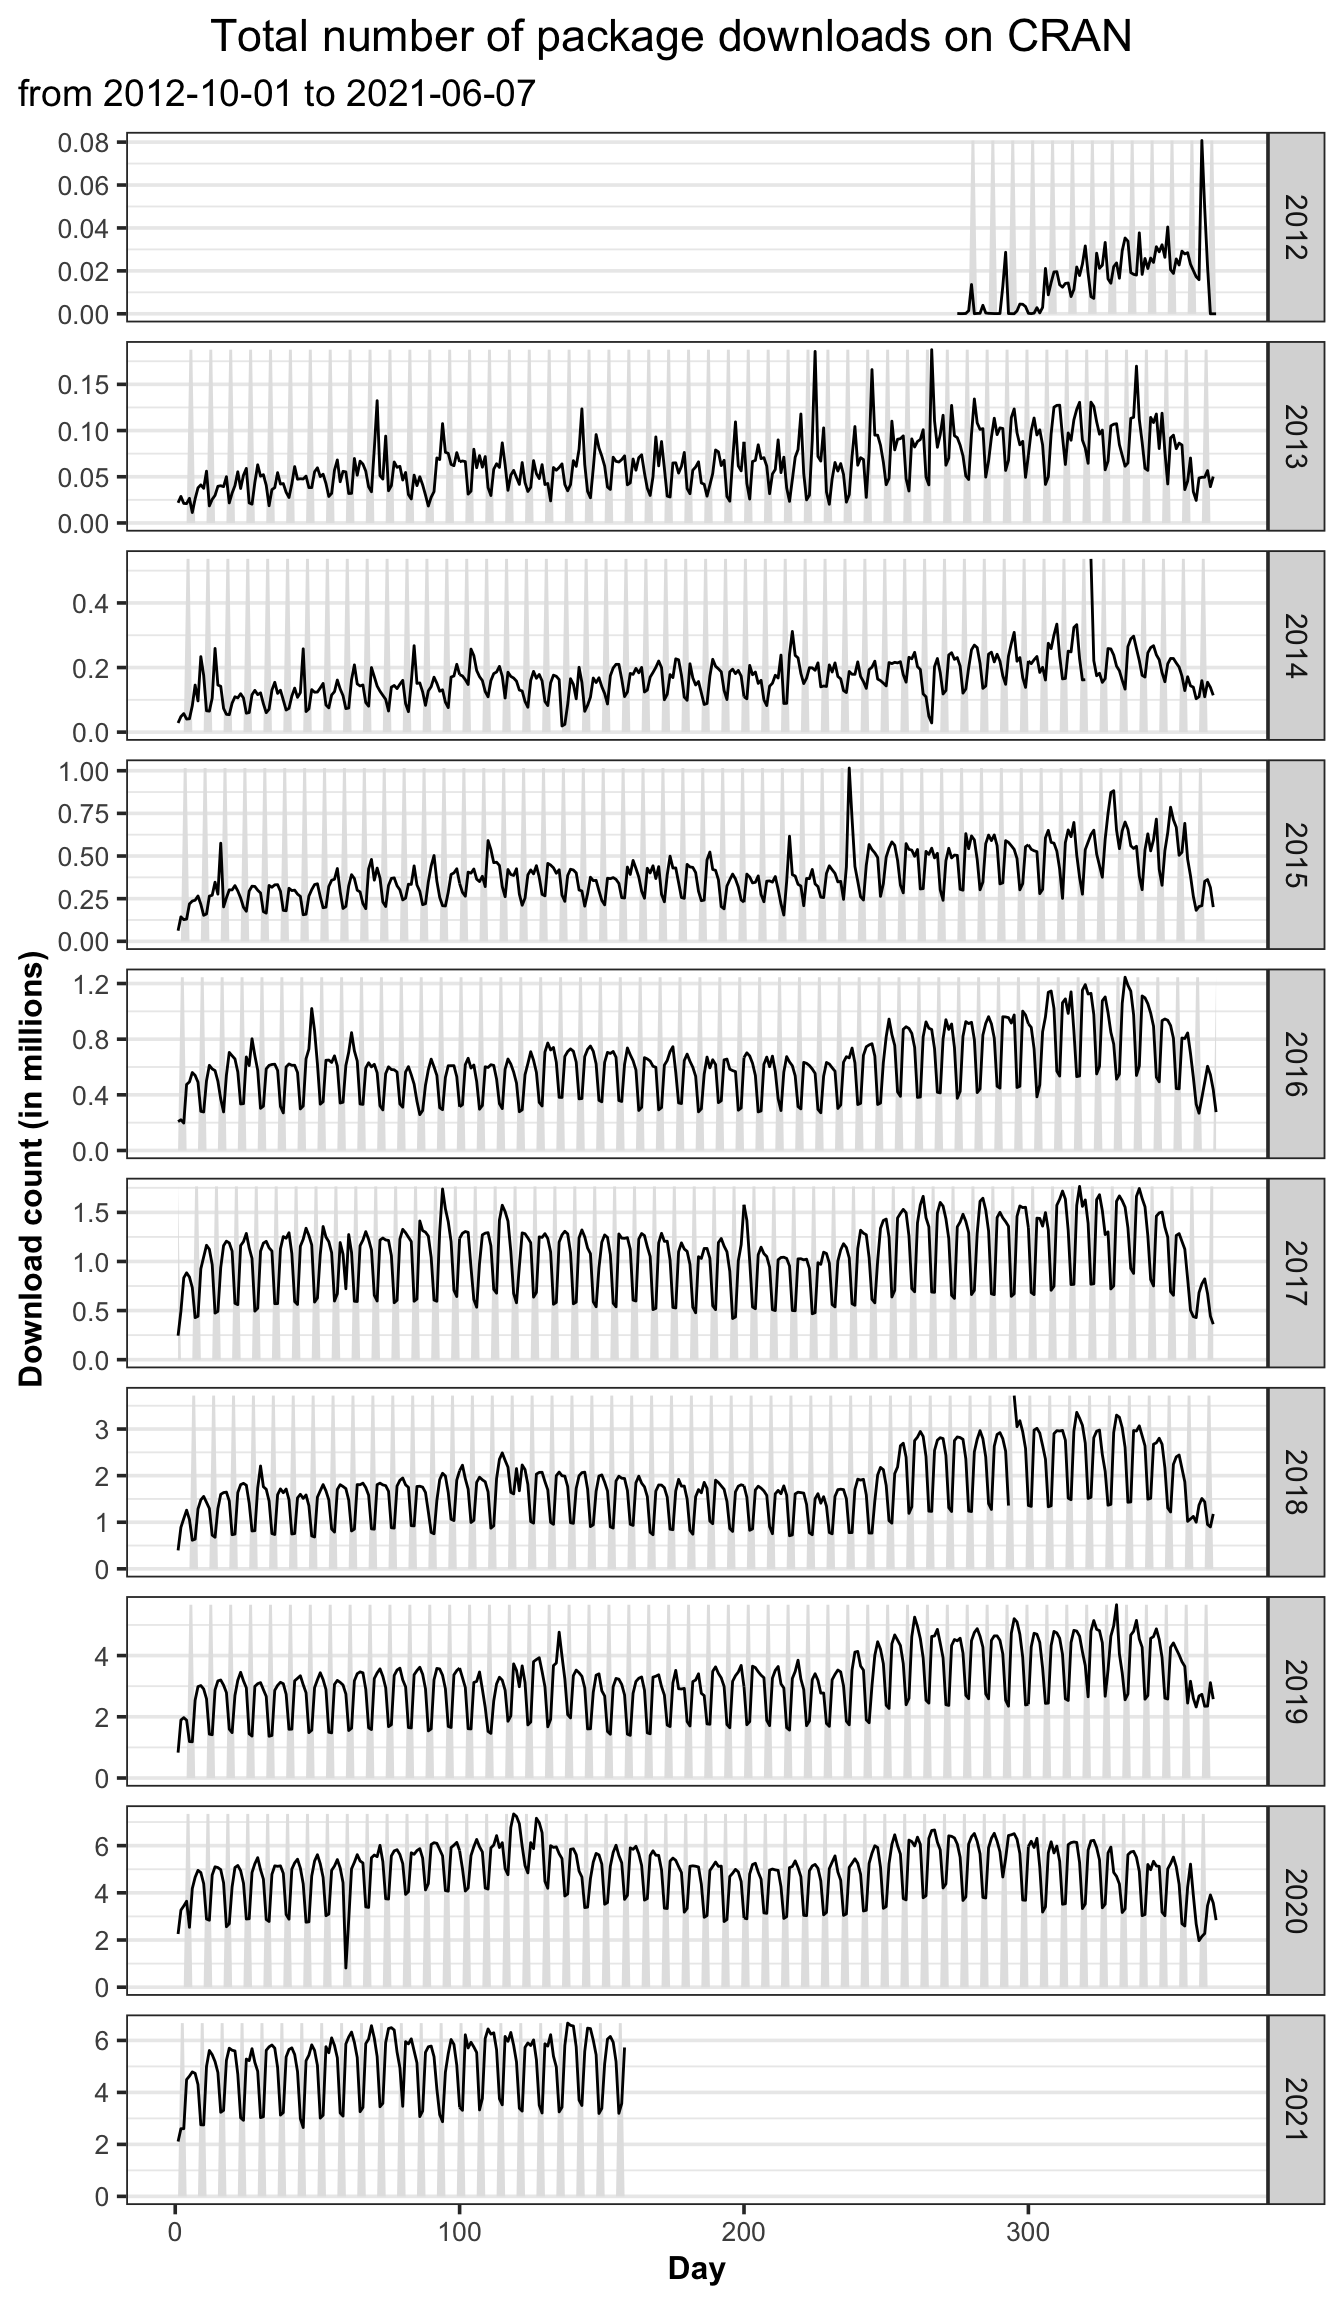
\includegraphics{figures/total-trend-1} 

}

\caption{The figure shows the total downloads of all R-packages on CRAN would decrease on weekends.}\label{fig:total-trend}
\end{figure}

As there are many fluctuation in daily download pattern which is due to calendar effect and server issue of CRAN mirror, we then applied a model called STL decomposition explained in \textcite{stl}, to smooth the curve for all the R-packages.



\begin{figure}

{\centering 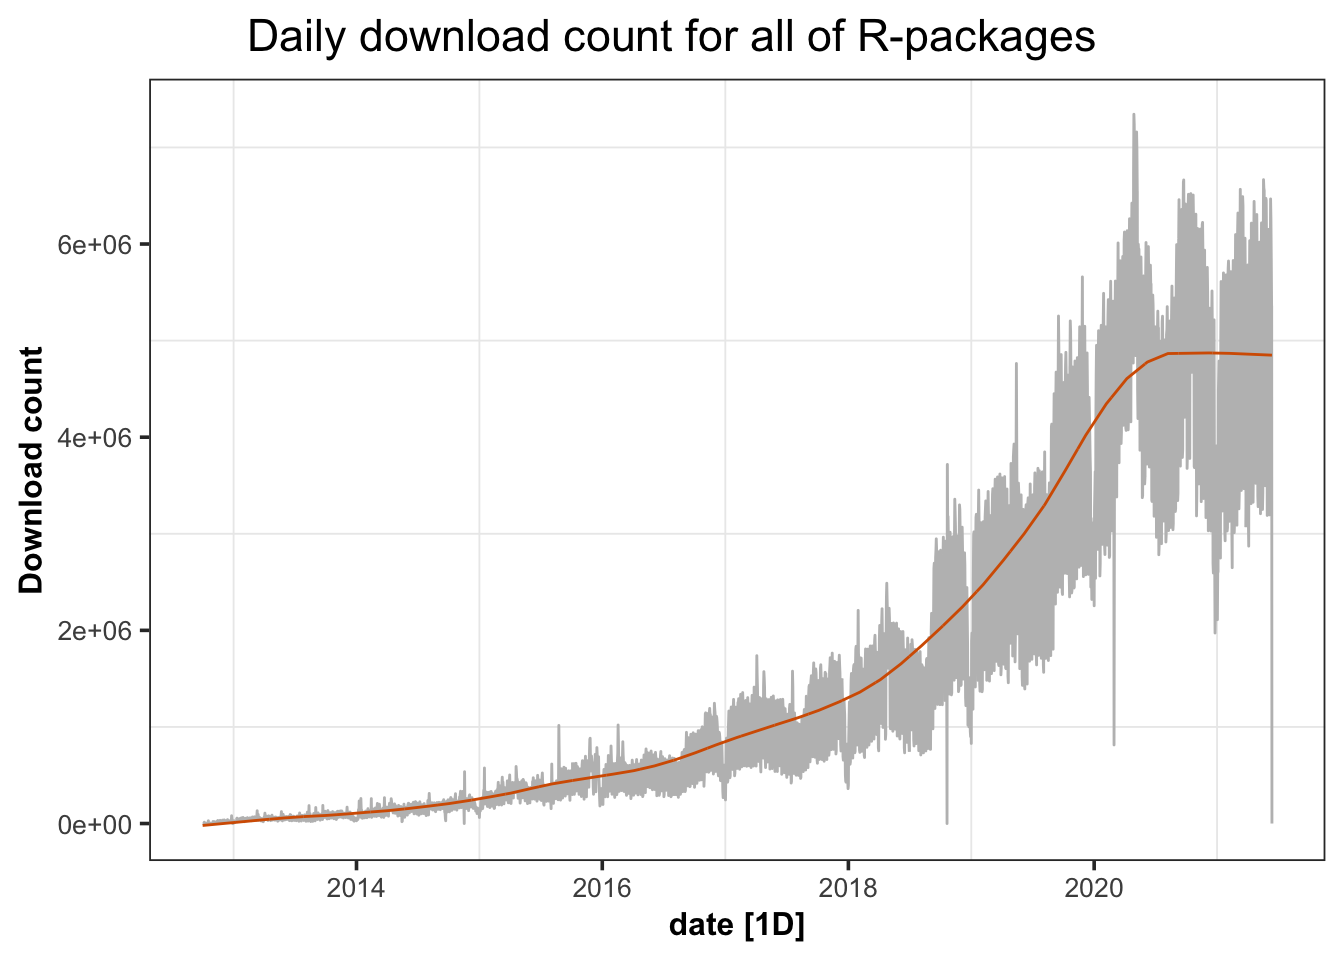
\includegraphics{figures/pkg-stl-1} 

}

\caption{The figure shows the total downloads of all R-packages on CRAN after smoothing.}\label{fig:pkg-stl}
\end{figure}

And this can be applied to any R-package to adjust the daily download pattern. In this case, we selected two packages \texttt{fable} and \texttt{forecast} as an example in Figure \ref{fig:example-adjust}. It can be seen that the pattern is smoother after removing the seasonality and ignorance of extremum possibly caused by repeated downloads, updates and test downloads from the server.



\begin{figure}

{\centering 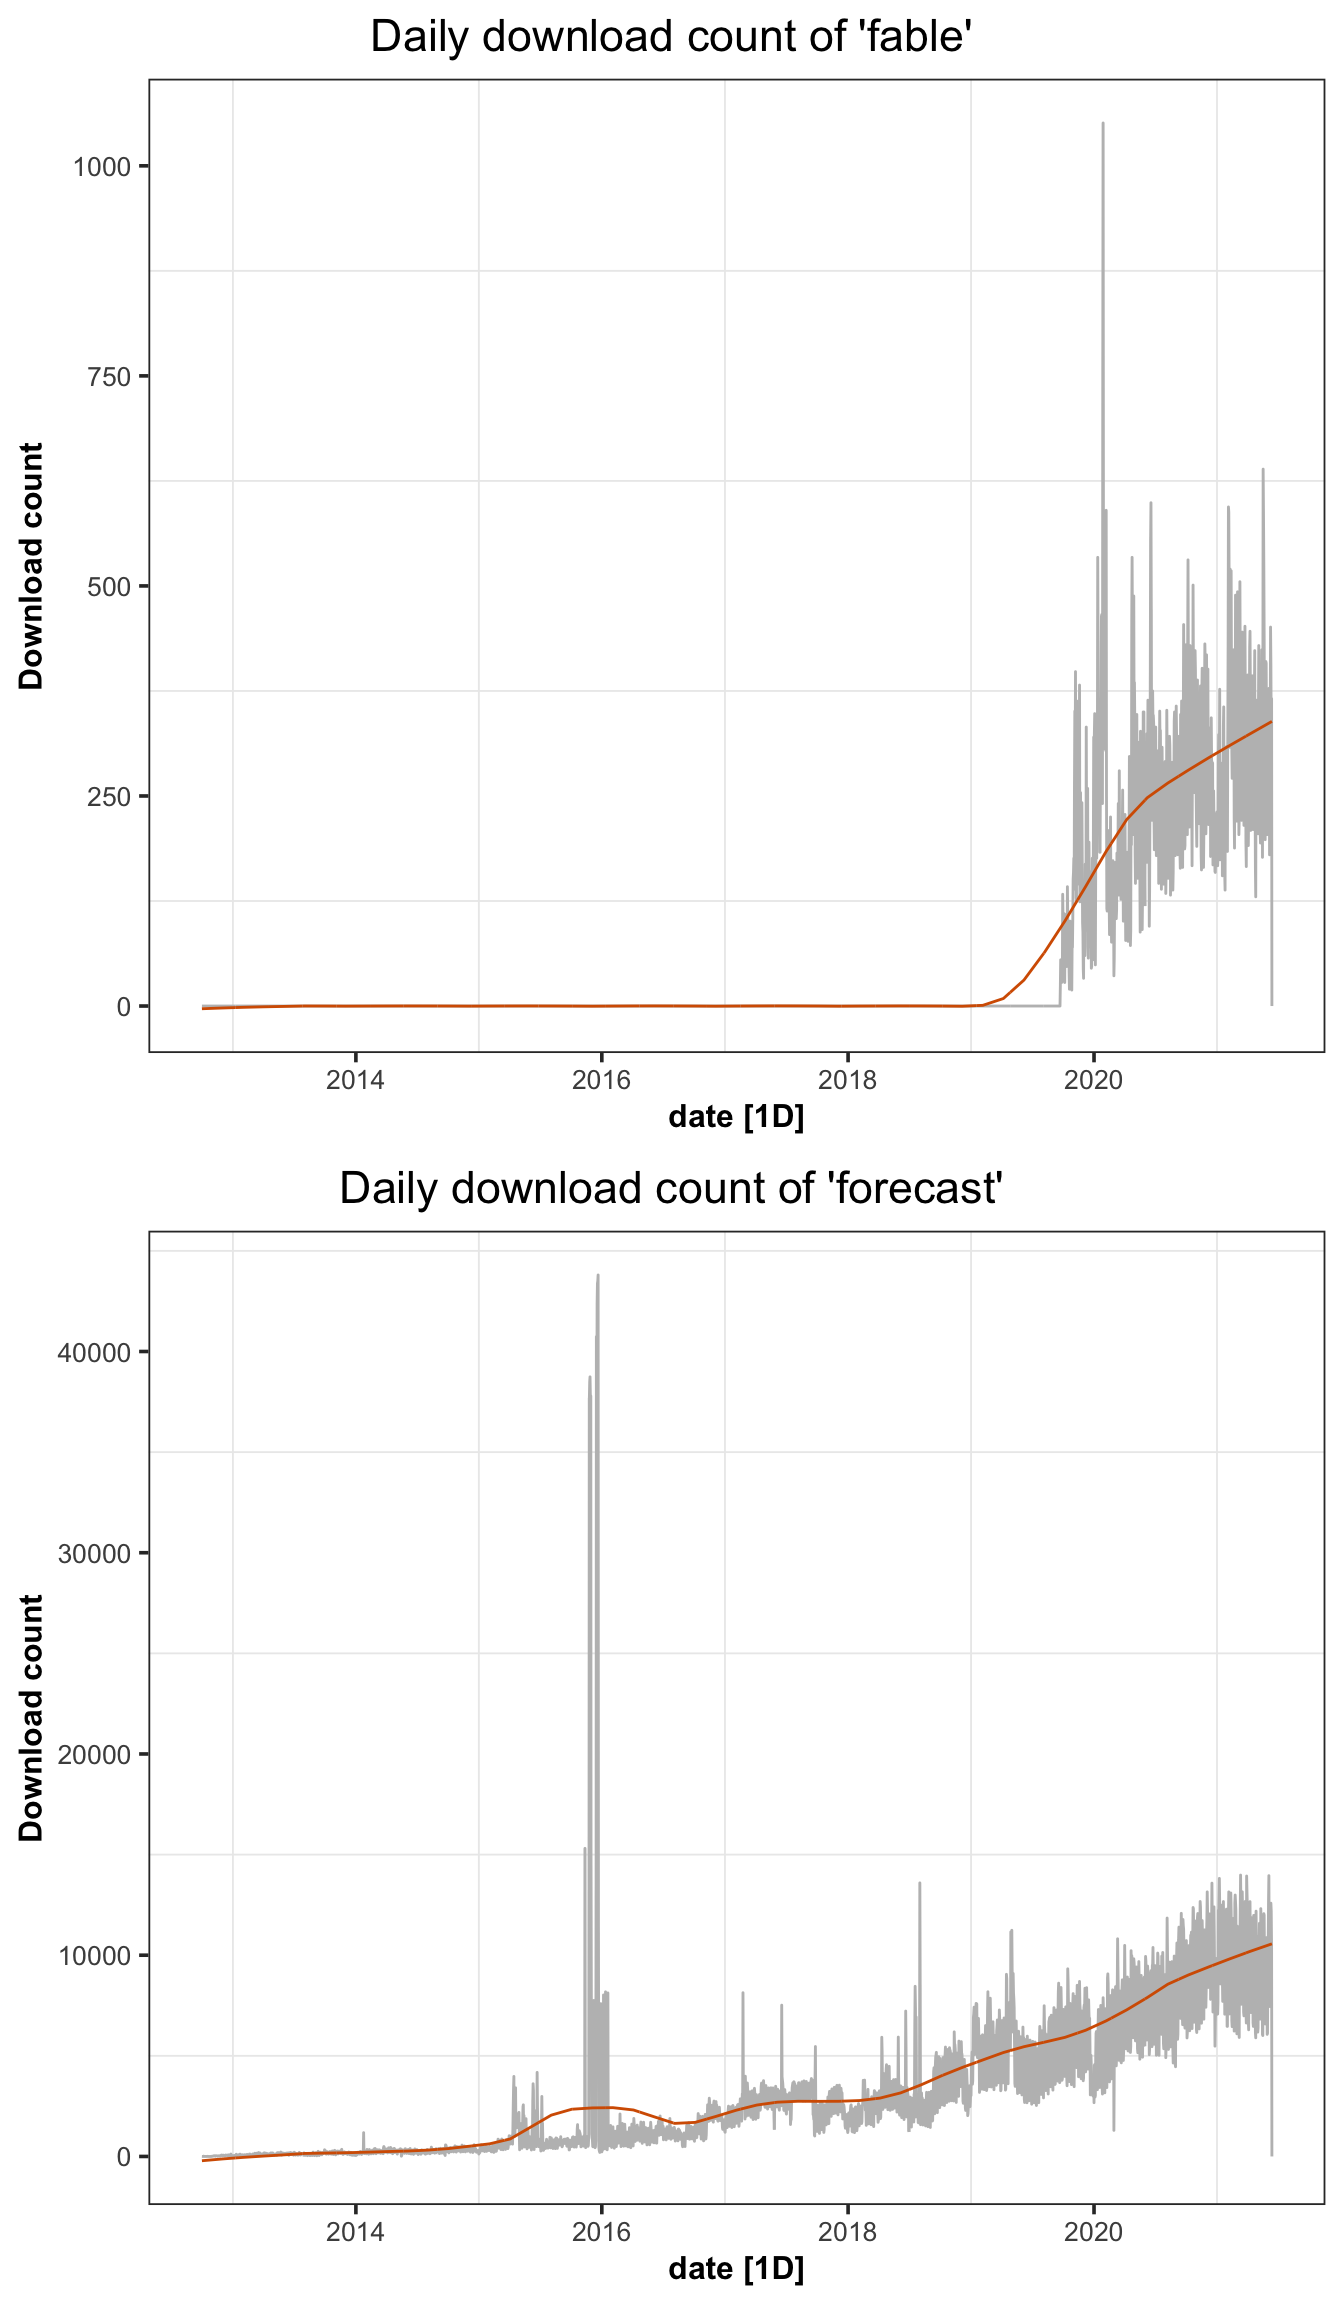
\includegraphics{figures/example-adjust-1} 

}

\caption{The figure shows the daily downloads of \texttt{fable} and \texttt{forecast} on CRAN after smoothing.}\label{fig:example-adjust}
\end{figure}

Figure \ref{fig:weekend-vs-weekday} shows the distribution and the median of the downloads between weekday and weekends. The distribution of weekdays and weekends are quite different. Weekends are wider and shorter, while weekdays are thinner and higher, because the total download of data on weekends is less than that on weekdays. And in 2012, the median and interquartile range of download logs are not very distinguished between weekdays and weekends, for the data volume was not adequate at this time as mentioned above. But after 2013, the gap between the two becomes more and more obvious, that is, the median downloads of working days is significantly higher than that of weekends, and the overall number of data is also significantly higher than that of weekends as well. But interestingly, the lower adjacent sometimes occurs on weekends, such as in year 2014, 2015, 2018, 2019 and 2021, while sometimes in weekdays, such as in year 2012, 2013, 2016, 2017 and 2020.

\begin{center}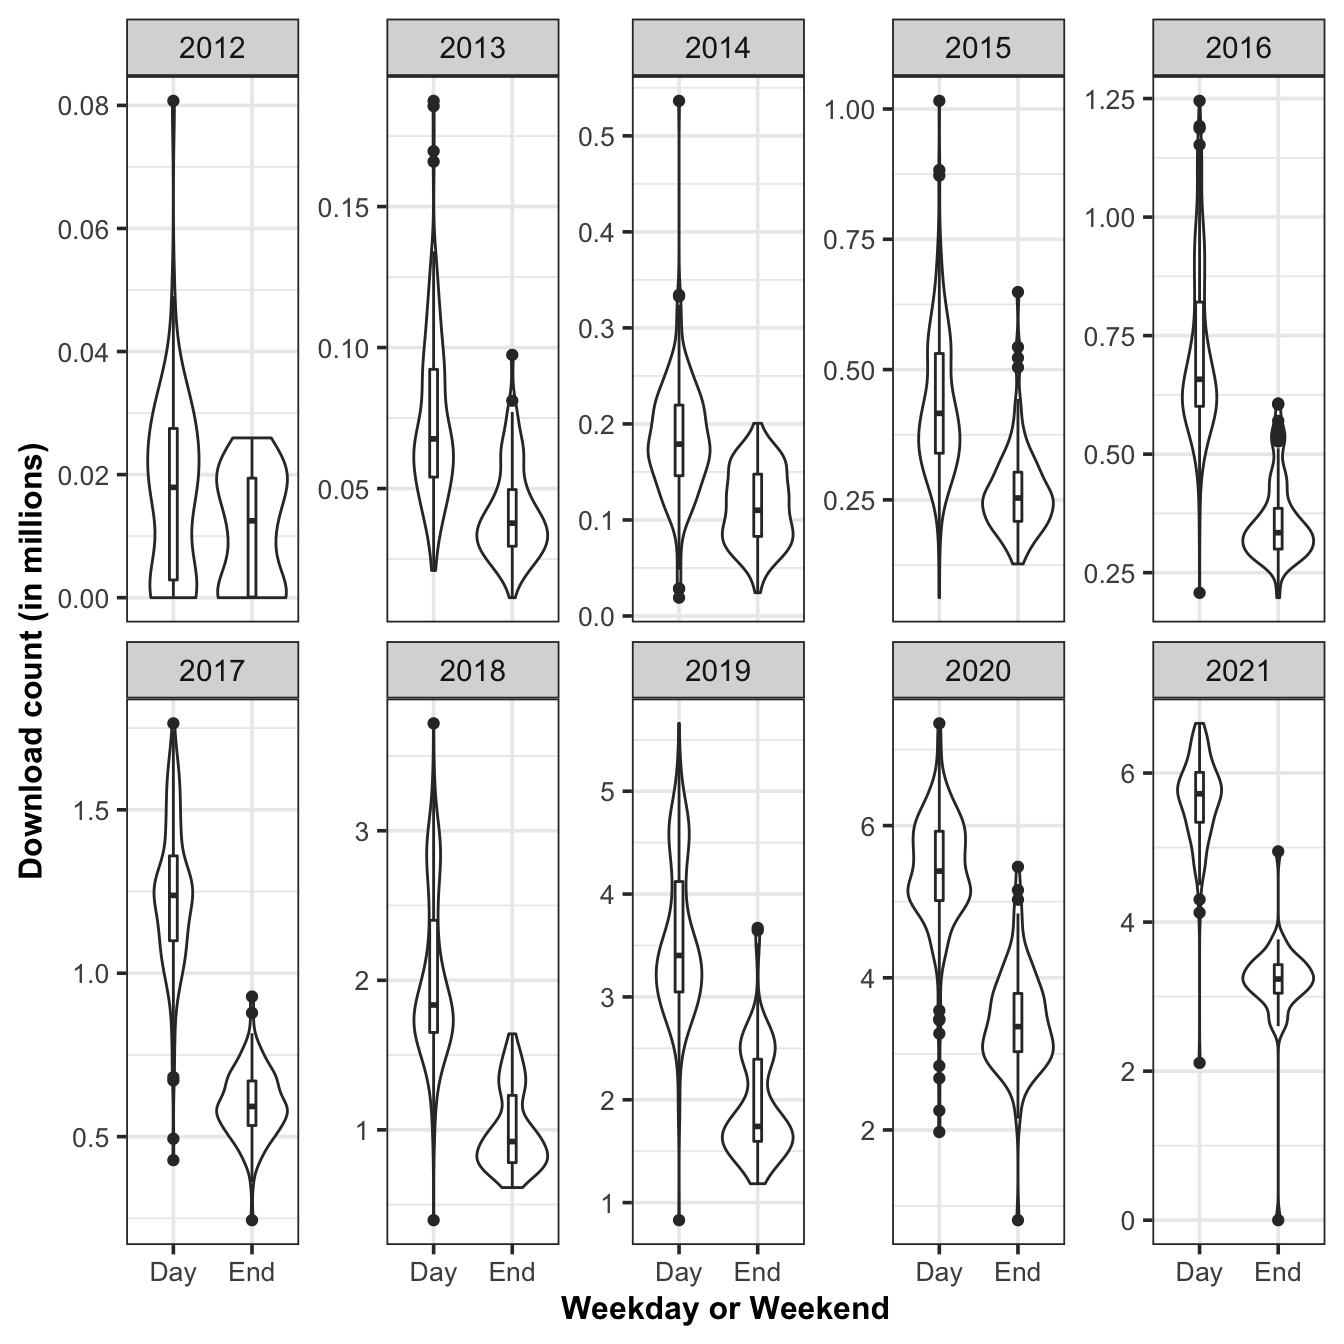
\includegraphics{figures/weekend-vs-weekday-1} \end{center}

\begin{discovery}
\textbf{Finding 4}: Top 10\% downloaded R-packages share nearly 90\%
cumulative download count of the whole.
\end{discovery}

From the previous analysis, we could see that the cumulative download count of R-packages shows an increasing trend. It would be perfect equality if every R-package had the same download count -- the last 20\% downloaded R-packages would gain 20\% of the total download count or the top 60\% downloaded R-packages would get 60\% of the total download count. But we know from experience that this is obviously impossible, so here we introduced Lorenz curve\autocite{lorenz} to show the respective number of R-packages of different download levels (groups defined by quantiles of download count). In this way, we could figure out how many download counts contributed by different downloaded R-packages.

Figure \ref{fig:download-over-time} shows cumulative download count against each downloaded group. It can be seen that most of the download counts come from the top 10\% downloaded R-packages. At the same time, we could also observe that the Gini value is close to 1, which indicates that the download volume among groups is very unbalanced. In fact, the download volume of the top 10\% group is extremely distinguished from that of the following groups. It's not hard to understand that this group should contain some R-packages with high popularity and large quantities of users. For example, if we extracted the first 10 packages of this group in Table \ref{tab:top10}, we could find that they are all quite famous and frequently-used ones.



\begin{figure}

{\centering 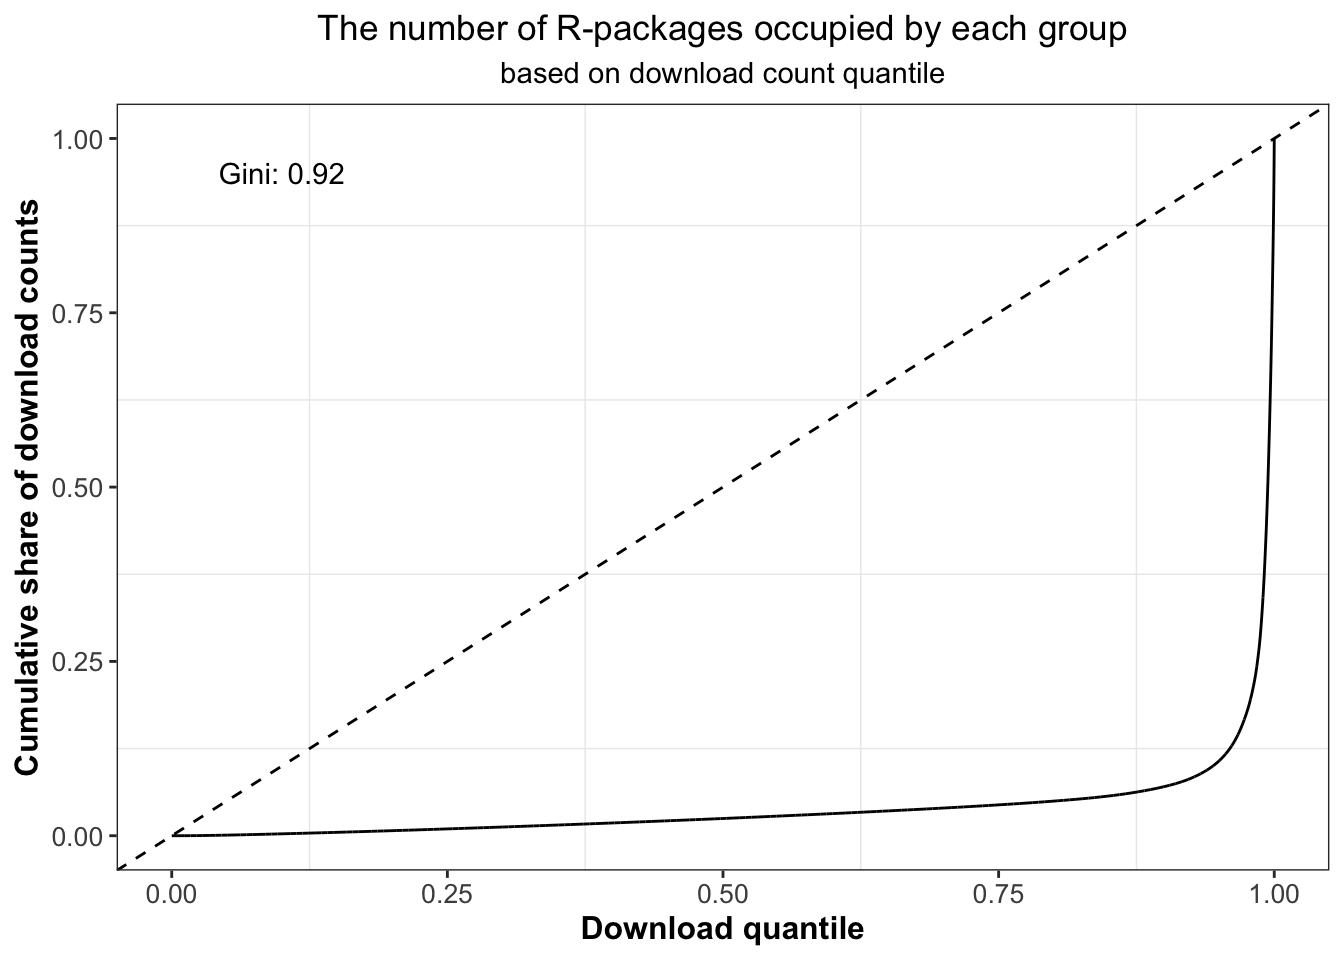
\includegraphics{figures/lorenz-all-1} 

}

\caption{Percentiles of the download count against cumulative download count of R-packages at or below that percentile.}\label{fig:lorenz-all}
\end{figure}

\textbackslash begin\{table\}

\textbackslash caption\{\label{tab:top10}First 10 R-packages of top 10\% downloaded group\}
\centering

\begin{tabular}[t]{l|r}
\hline
package & total\\
\hline
rlang & 15572507\\
\hline
vctrs & 13544857\\
\hline
dplyr & 12739206\\
\hline
ggplot2 & 12670952\\
\hline
jsonlite & 12627542\\
\hline
lifecycle & 11124212\\
\hline
tibble & 10935860\\
\hline
magrittr & 10312021\\
\hline
pillar & 9566463\\
\hline
glue & 9534999\\
\hline
\end{tabular}

\textbackslash end\{table\}

\hypertarget{daily-downloads-of-r}{%
\section{Daily downloads of R}\label{daily-downloads-of-r}}

In this section, we studied the daily downloads of R language itself from 2012-10-01 to 2021-06-07. The data was obtained from the \texttt{cranlogs} package \autocite{cranlogs} as well.

\begin{discovery}
\textbf{Finding 1}: The number of downloads shows an upward trend over
time, and the variance also increases with the downloads.
\end{discovery}

Figure \ref{fig:R-download-trend} shows the download trend of R on CRAN over time. It shows an upward trend over time, and the variance also increases with the download count, which indicates the volatility of the data is increasing as well. And that is resulted from the pump of R users. As for the significant spikes, it is probably quite similar to the situation of R-packages, which is due to repeated downloads, weekly calendar effect and server test.



\begin{figure}

{\centering 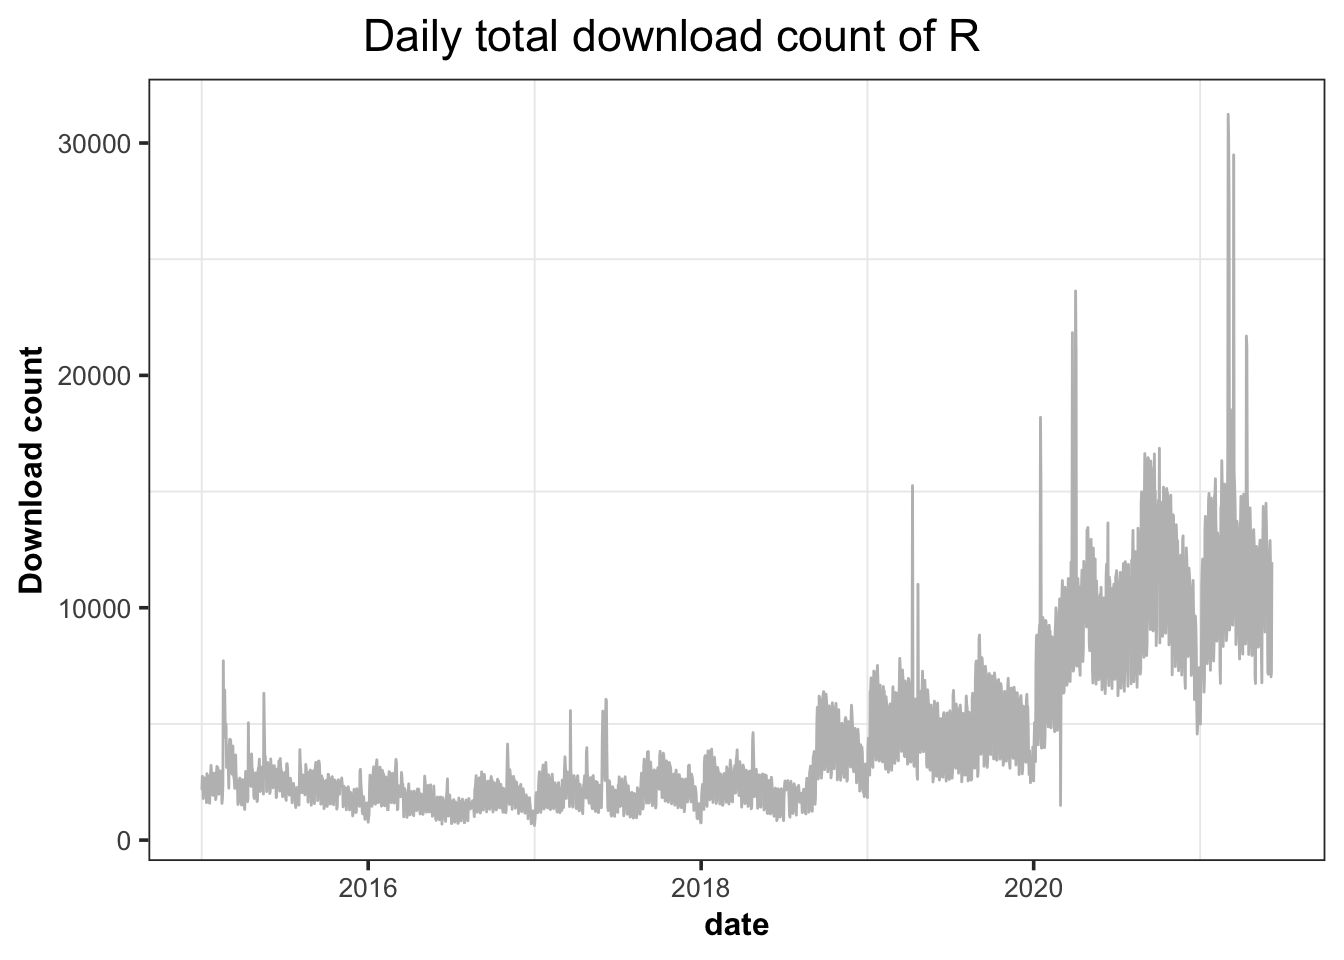
\includegraphics{figures/R-download-trend-1} 

}

\caption{The download trend of R on CRAN over time.}\label{fig:R-download-trend}
\end{figure}

\begin{discovery}
\textbf{Finding 2}: The most used operation system for R users is
Windows OS.
\end{discovery}

Figure \ref{fig:R-download-trend-os} shows the comparison of operation system for R users. The number of Windows users ranks first, followed by MacOS and SRC. For Microsoft has traditionally dominated the desktop and laptop market. And Microsoft officially claims there are 400 million active users of Windows 10 itself, while Apple revealed that there are now nearly 100 million active Mac users.\autocite{warren2017}



\begin{figure}

{\centering 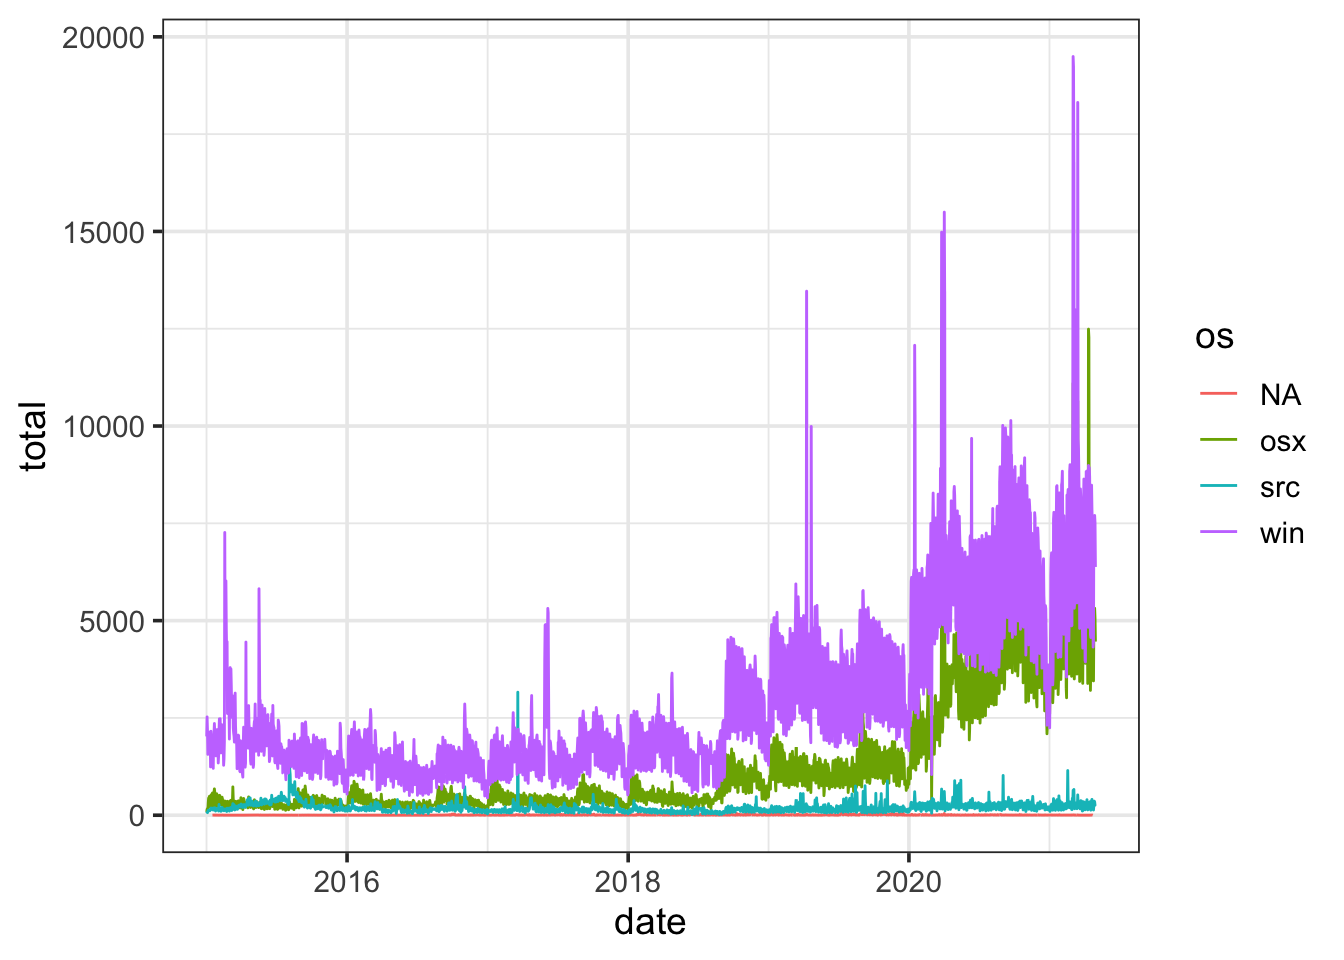
\includegraphics{figures/R-download-trend-os-1} 

}

\caption{The download trend of R on CRAN over time.}\label{fig:R-download-trend-os}
\end{figure}

\begin{discovery}
\textbf{Finding 3}: The most popular version of R is 3.2.1
\end{discovery}

And Table \ref{tab:R-download-trend-version} shows the number of downloads of different versions of R. The most downloaded one is 3.2.1 with 4526 times, followed by 3.3.3 with 4305 times and 3.1.2 with 3958 times. So, most users tend to install the latest version of R to get the newest update information.

\begin{table}

\caption{\label{tab:R-download-trend-version}The number of downloads of different versions of R}
\centering
\begin{tabular}[t]{l|r}
\hline
R\_version & count\\
\hline
3.2.1 & 4526\\
\hline
3.3.3 & 4305\\
\hline
3.1.2 & 3958\\
\hline
3.2.2 & 3781\\
\hline
3.4.0 & 3585\\
\hline
3.1.1 & 3458\\
\hline
3.5.1 & 3450\\
\hline
3.4.3 & 3409\\
\hline
3.4.1 & 3398\\
\hline
3.3.0 & 3362\\
\hline
3.4.4 & 3349\\
\hline
3.2.3 & 3308\\
\hline
3.0.3 & 3294\\
\hline
3.1.3 & 3274\\
\hline
3.3.2 & 3235\\
\hline
3.1.0 & 3216\\
\hline
3.5.0 & 3136\\
\hline
3.3.1 & 3107\\
\hline
2.15.3 & 2895\\
\hline
3.2.0 & 2873\\
\hline
3.4.2 & 2743\\
\hline
3.6.1 & 2636\\
\hline
3.0.1 & 2543\\
\hline
3.0.0 & 2537\\
\hline
3.0.2 & 2517\\
\hline
3.5.2 & 2514\\
\hline
3.5.3 & 2496\\
\hline
3.6.0 & 2374\\
\hline
2.15.0 & 2203\\
\hline
3.2.4 & 2122\\
\hline
2.15.1 & 2066\\
\hline
2.13.2 & 2011\\
\hline
3.2.5 & 1981\\
\hline
2.15.2 & 1906\\
\hline
devel & 1856\\
\hline
3.6.2 & 1807\\
\hline
2.14.1 & 1791\\
\hline
2.11.1 & 1764\\
\hline
2.11.0 & 1733\\
\hline
2.14.2 & 1700\\
\hline
2.14.0 & 1660\\
\hline
2.13.0 & 1628\\
\hline
2.13.1 & 1585\\
\hline
3.6.3 & 1560\\
\hline
2.10.0 & 1496\\
\hline
2.10.1 & 1476\\
\hline
2.12.0 & 1432\\
\hline
2.12.2 & 1387\\
\hline
2.12.1 & 1362\\
\hline
4.0.0 & 1346\\
\hline
4.0.1 & 1251\\
\hline
4.0.3 & 1092\\
\hline
4.0.2 & 1071\\
\hline
3.6.2.nn & 508\\
\hline
3.2.4revised & 480\\
\hline
3.6.3.nn & 459\\
\hline
4.0.4 & 443\\
\hline
release & 407\\
\hline
2.9.2 & 394\\
\hline
4.0.5 & 334\\
\hline
2.9.0 & 314\\
\hline
2.8.1 & 312\\
\hline
2.0.0 & 309\\
\hline
2.5.1 & 300\\
\hline
2.5.0 & 296\\
\hline
2.9.1 & 293\\
\hline
2.8.0 & 292\\
\hline
2.1.1 & 290\\
\hline
2.2.0 & 290\\
\hline
2.7.0 & 290\\
\hline
2.4.1 & 284\\
\hline
2.6.0 & 282\\
\hline
2.2.1 & 277\\
\hline
2.4.0 & 274\\
\hline
2.7.1 & 272\\
\hline
2.6.2 & 267\\
\hline
2.3.1 & 265\\
\hline
2.3.0 & 254\\
\hline
2.7.2 & 251\\
\hline
2.6.1 & 248\\
\hline
2.1.0 & 232\\
\hline
3.6.1patched & 228\\
\hline
2.0.1 & 208\\
\hline
3.5.1patched & 144\\
\hline
patched.exe & 141\\
\hline
release.exe & 138\\
\hline
4.0.3patched & 132\\
\hline
4.0.2patched & 120\\
\hline
3.5.2patched & 99\\
\hline
3.6.2patched & 96\\
\hline
3.6.0patched & 85\\
\hline
3.3.2patched & 75\\
\hline
3.2.2patched & 71\\
\hline
3.3.1patched & 70\\
\hline
3.2.3patched & 69\\
\hline
4.1.0 & 61\\
\hline
3.4.1patched & 58\\
\hline
3.4.3patched & 55\\
\hline
3.6.3patched & 55\\
\hline
3.1.2patched & 54\\
\hline
3.5.3patched & 53\\
\hline
3.2.0patched & 50\\
\hline
4.0.5patched & 49\\
\hline
4.0.0patched & 47\\
\hline
3.4.0patched & 46\\
\hline
4.0.4patched & 45\\
\hline
2.2.1pat & 42\\
\hline
3.2.1patched & 41\\
\hline
3.1.3patched & 37\\
\hline
3.4.2patched & 35\\
\hline
3.3.3patched & 32\\
\hline
3.5.0patched & 30\\
\hline
3.3.0patched & 29\\
\hline
3.2.4-revised & 22\\
\hline
4.0.3rc & 22\\
\hline
3.2.4patched & 20\\
\hline
4.1.0patched & 20\\
\hline
3.6.0alpha & 19\\
\hline
4.0.0alpha & 18\\
\hline
3.3.0beta & 17\\
\hline
4.0.1patched & 17\\
\hline
3.1.3rc & 14\\
\hline
3.2.1rc & 14\\
\hline
4.1.0alpha & 14\\
\hline
3.2.0alpha & 13\\
\hline
3.2.0rc & 12\\
\hline
3.2.2rc & 11\\
\hline
3.6.1rc & 11\\
\hline
4.0.1rc & 11\\
\hline
3.4.0alpha & 10\\
\hline
3.6.0rc & 10\\
\hline
3.6.3beta & 10\\
\hline
4.0.4rc & 10\\
\hline
3.4.4patched & 9\\
\hline
3.5.0alpha & 9\\
\hline
3.5.3rc & 9\\
\hline
3.6.2rc & 9\\
\hline
4.0.2rc & 9\\
\hline
4.1.0rc & 9\\
\hline
3.2.0beta & 8\\
\hline
3.2.5patched & 8\\
\hline
3.4.4rc & 8\\
\hline
3.5.0rc & 8\\
\hline
3.6.0beta & 8\\
\hline
4.0.0rc & 8\\
\hline
4.0.3beta & 8\\
\hline
3.3.3rc & 7\\
\hline
3.6.3rc & 7\\
\hline
4.1.0beta & 7\\
\hline
3.2.3rc & 6\\
\hline
3.2.4rc & 6\\
\hline
3.3.1rc & 6\\
\hline
3.5.2rc & 6\\
\hline
3.6.1beta & 6\\
\hline
4.0.0beta & 6\\
\hline
4.0.1beta & 6\\
\hline
3.2.2beta & 5\\
\hline
3.4.0beta & 5\\
\hline
3.3.0alpha & 4\\
\hline
3.3.0rc & 4\\
\hline
3.3.2rc & 4\\
\hline
3.4.0rc & 4\\
\hline
3.4.1rc & 4\\
\hline
3.4.2rc & 4\\
\hline
3.4.3rc & 4\\
\hline
4.0.5beta & 4\\
\hline
4.0.5rc & 4\\
\hline
3.1.3beta & 3\\
\hline
3.2.1beta & 3\\
\hline
3.4.3beta & 3\\
\hline
3.5.0beta & 3\\
\hline
3.6.2beta & 3\\
\hline
4.0.2beta & 3\\
\hline
4.0.4beta & 3\\
\hline
3.2.3beta & 2\\
\hline
3.2.4beta & 2\\
\hline
3.3.1beta & 2\\
\hline
3.4.1beta & 2\\
\hline
3.5.1rc & 2\\
\hline
3.5.2beta & 2\\
\hline
3.4.2beta & 1\\
\hline
3.5.3beta & 1\\
\hline
devel.exe & 1\\
\hline
\end{tabular}
\end{table}

In conclusion, the daily download trend of R is quite similar to that of R-packages, and they are both significantly affected by weekly calendar issue, unusual downloads from CRAN mirrors. But in general, they both tend to increase with the growing of R users.

\hypertarget{daily-top-15-downloaded-r-packages}{%
\section{Daily top 15 downloaded R-packages}\label{daily-top-15-downloaded-r-packages}}

In this section, we studied the top 15 downloaded R-packages from 2013-04-01 to 2021-04-01 to see how user preferences has been changing. The data was obtained from CRAN website {[}\url{http://cran.rstudio.com/web/packages/packages.rds}{]}.

We are supposed to know that some R-packages are hold by Rstudio, and some are developed by core personnel or personnel closely related to R, or some prolific developers. Naturally, the number of downloads of these packages will probably be higher. On the one hand, the R-packages developed by these experienced developers may be more mature and perfect, on the other hand, users are more inclined to use the packages from famous authors, which can be regarded as a kind of ``good use'' guarantee.

However, the existence of these packages will make the results biased. Therefore, in order to explore the R-packages constructed by non-special creators, we have screened out four types of R-packages, namely:

\begin{itemize}
\tightlist
\item
  R-packages maintained by R studio
\item
  R-packages created by authors from R core group
\item
  R-packages created by authors from R secondary group
\item
  R-packages created by R related authors
\item
  R-packages created by top 20 prolific maintainers (This is resourced at \textcite{revolutions})
\end{itemize}

And after that, we generated the lorenz curve here again in Figure \ref{fig:lorenz-filter}, it can be observed that the distribution of R-packages in each download group is quite equal now and the Gini value decreases a lot as well, for the `extreme effect' brought by highly-downloaded packages has disappeared. Thus, the user preferences could be shown more clearly. But as after filtering, the number of remaining packages is only 58, which is a too small-sized sample to construct representative conclusions, we would still focus on all the R-packages on CRAN in our later analysis.



\begin{figure}

{\centering 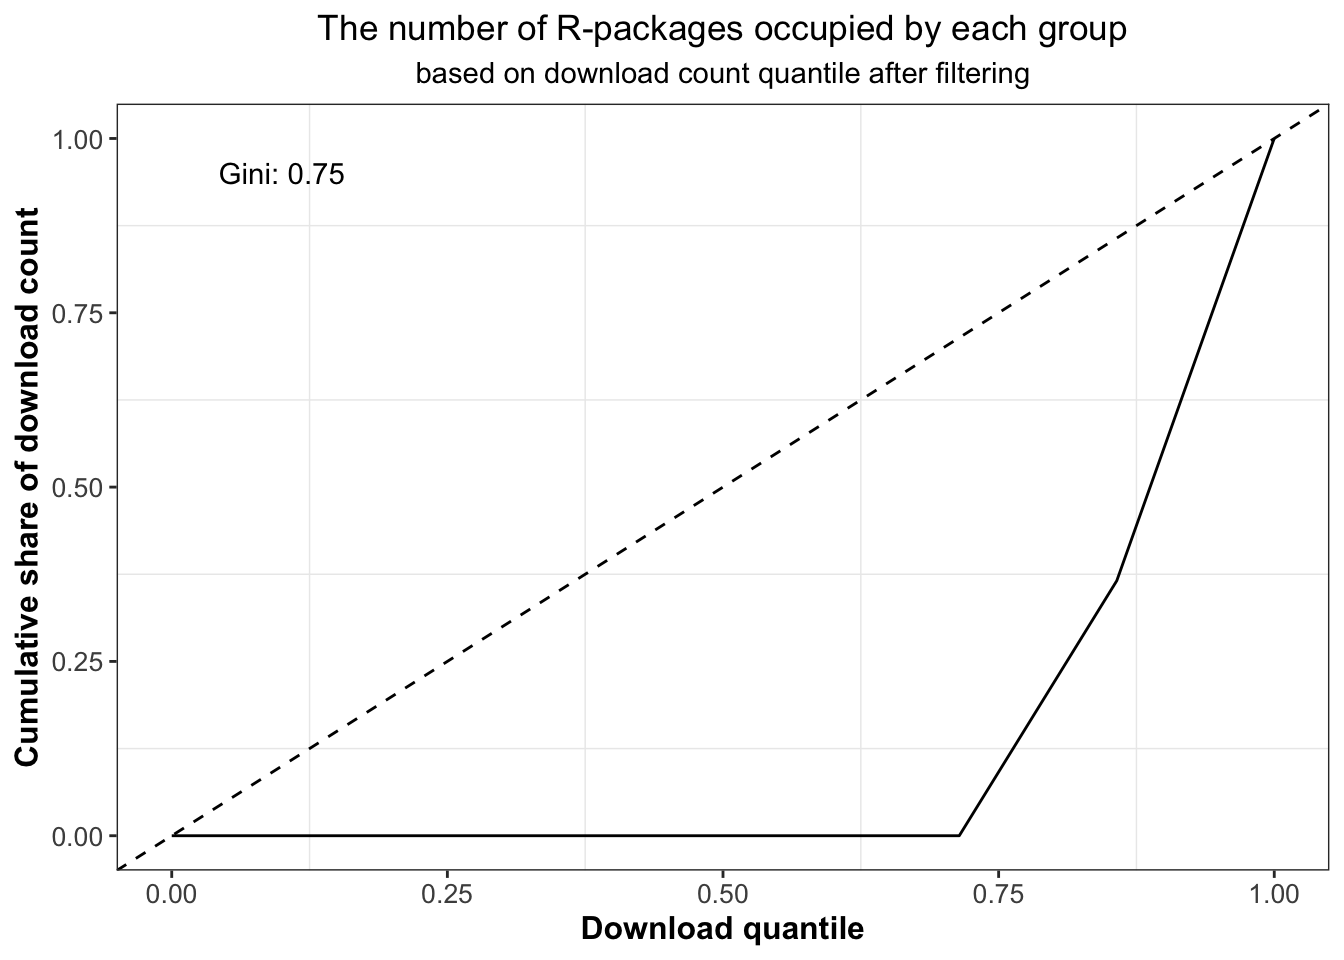
\includegraphics{figures/lorenz-filter-1} 

}

\caption{Percentiles of the download count against cumulative download count of R-packages after filtering four types of popular and highly-downloaded packages.}\label{fig:lorenz-filter}
\end{figure}

\begin{discovery}
\textbf{Finding 1}: The topic of newly added R-packages each year come
from quite different areas.
\end{discovery}

Table \ref{tab:changed-top15pkg} shows the R-packages that newly come up to the top 15 list each year, from which we can know how the user preference has changed year by year, compared with the previous year. To be more specific :

\begin{itemize}
\tightlist
\item
  For 2014, \texttt{ncdf} ranks first, which is used to provide an interface to netCDF format data.
\item
  For 2015, the first downloaded is \texttt{XLConnectJars} on JAVA dependency.
\item
  For 2016, the first one is \texttt{reports} for standardising the output of R.
\item
  For 2017, \texttt{lava.tobit} aims to help with estimation and simulation of latent variable models.
\item
  For 2018, the ranking-first \texttt{ReportsRs} is for creating Microsoft Word and Powerpoint documents.
\item
  For 2019, \texttt{CALIBERrfimpute} is used to impute missing values in analysis datasets using full conditional specifications.
\item
  For 2020, \texttt{SparkR} is similar to \texttt{dplyr} but for large datasets.
\item
  For 2021, \texttt{heatmap.plus} is an extension of \texttt{heatmap()} function.
\end{itemize}

\begin{table}

\caption{\label{tab:changed-top15pkg}Changed top 15 downloaded R-packages from 2013 to 2019}
\centering
\begin{tabular}[t]{l|l|l|l|l|l|l|l}
\hline
package14\_13 & package15\_14 & package16\_15 & package17\_16 & package18\_17 & package19\_18 & package20\_19 & package21\_20\\
\hline
ncdf & XLConnectJars & reports & lava.tobit & ReporteRs & freetypeharfbuzz & ENmisc & heatmap.plus\\
\hline
playwith & KoNLP & moonsun & rggobi & OceanView & replyr & CoxBoost & lazyrmd\\
\hline
DMwR & doRedis & rPython & alr3 & ReporteRsjars & zipcode & gWidgetstcltk & packagedocs\\
\hline
latticist & ElemStatLearn & rmongodb & tnam & gWidgetsRGtk2 & rmosek & citr & robcp\\
\hline
bstats & testthatsomemore & maxent & SweaveListingUtils & d3heatmap & msgpack & EMMIXskew & skedastic\\
\hline
geoRglm & adehabitat & SDMTools & ElemStatLearn & - & - & RcmdrPlugin.mosaic & nws\\
\hline
reports & wmtsa & MSBVAR & zipcode & - & - & RcmdrPlugin.qual & optimbase\\
\hline
- & mixOmics & d3heatmap & - & - & - & OceanView & SpaDES\\
\hline
- & DatABEL & ReporteRs & - & - & - & - & SpaDES.core\\
\hline
- & - & - & - & - & - & - & bomrang\\
\hline
- & - & - & - & - & - & - & snipEM\\
\hline
- & - & - & - & - & - & - & SpaDES.addins\\
\hline
- & - & - & - & - & - & - & swissdd\\
\hline
\end{tabular}
\end{table}

\begin{discovery}
\textbf{Finding 2}: The topic of R-packages changes least between 2017
and 2019. And the most popular filed is about JAVA dependency.
\end{discovery}

Table \ref{tab:unchanged-top15pkg} shows the R-packages that remain unchanged each year compared with the previous year, from which we can know which packages are relatively stable in popularity.

To be more specific, packages like \texttt{XLConnectJars}, \texttt{DMwR}, \texttt{KoNLP}, and \texttt{gWidgets} are relatively popular through years from 2014 to 2021. And they are used for providing JAVA dependency, data mining, linguistic research and providing API for building toolkit-independent, interactive GUIs.

\begin{table}

\caption{\label{tab:unchanged-top15pkg}Unchanged top 15 downloaded R-packages from 2013 to 2019}
\centering
\begin{tabular}[t]{l|l|l|l|l|l|l|l}
\hline
package14\_13 & package15\_14 & package16\_15 & package17\_16 & package18\_17 & package19\_18 & package20\_19 & package21\_20\\
\hline
Defaults & ncdf & XLConnectJars & XLConnectJars & XLConnectJars & XLConnectJars & freetypeharfbuzz & freetypeharfbuzz\\
\hline
RSQLite.extfuns & epicalc & KoNLP & KoNLP & DMwR & KoNLP & DMwR & OceanView\\
\hline
gWidgetsRGtk2 & gWidgets & DMwR & DMwR & KoNLP & DMwR & gWidgets & -\\
\hline
gWidgets & gWidgetsRGtk2 & gWidgets & reports & SDMTools & SDMTools & d3heatmap & -\\
\hline
alr3 & DMwR & mixOmics & maxent & reports & gWidgets & alr3 & -\\
\hline
epicalc & alr3 & gWidgetsRGtk2 & SDMTools & mixOmics & ElemStatLearn & gWidgetsRGtk2 & -\\
\hline
rggobi & - & - & mixOmics & ElemStatLearn & reports & reports & -\\
\hline
its & - & - & gWidgets & alr3 & gWidgetsRGtk2 & - & -\\
\hline
- & - & - & - & maxent & d3heatmap & - & -\\
\hline
- & - & - & - & gWidgets & alr3 & - & -\\
\hline
\end{tabular}
\end{table}

Let's take a look at the trending R-packages. Trending R-packages are ones that are downloaded at least 1000 times last week, which have increased significantly compared to the average weekly downloads in the previous 24 weeks\autocite{r-hub}. That is to say, they are packages with high download volume in a recent short time. Through their topic, we can know what areas of R-packages people are concerned about recently.

\begin{discovery}
\textbf{Finding 3}: The most popular topic of trending R-packages is for
\texttt{r\ pkg\_trendcom\_count\$topic{[}1{]}}.
\end{discovery}

Table \ref{tab:trending-topic} shows the first 15 trending R-packages along with their topics.

\begin{table}

\caption{\label{tab:trending-topic}Trending R-packages with topics}
\centering
\begin{tabular}[t]{l|l}
\hline
package & topic\\
\hline
mgcv & Bayesian\\
\hline
units & ChemPhys\\
\hline
metafor & ClinicalTrials\\
\hline
clusterSim & Cluster\\
\hline
fastcluster & Cluster\\
\hline
lhs & Distributions\\
\hline
mgcv & Econometrics\\
\hline
mgcv & Environmetrics\\
\hline
DiceDesign & ExperimentalDesign\\
\hline
lhs & ExperimentalDesign\\
\hline
Cubist & MachineLearning\\
\hline
metafor & MetaAnalysis\\
\hline
norm & MissingData\\
\hline
arulesSequences & ModelDeployment\\
\hline
clusterSim & Multivariate\\
\hline
\end{tabular}
\end{table}

And Table \ref{tab:trending-count} shows the first 10 topics for trending R-packages. The most popular topic is Bayesian, followed by Cluster and Econometrics. This is easy to understand, because the number of users from different fields is different, so there are also differences in the number of R-packages used in different topics. And it seems that Bayesian is quite a hit recently.

\begin{table}

\caption{\label{tab:trending-count}Topics of trending R-packages}
\centering
\begin{tabular}[t]{l|r}
\hline
topic & download times\\
\hline
WebTechnologies & 5\\
\hline
Multivariate & 4\\
\hline
MachineLearning & 3\\
\hline
SocialSciences & 3\\
\hline
TimeSeries & 3\\
\hline
Cluster & 2\\
\hline
Econometrics & 2\\
\hline
MissingData & 2\\
\hline
OfficialStatistics & 2\\
\hline
Optimization & 2\\
\hline
\end{tabular}
\end{table}

So, apart from the topic of the R-package itself, what other factors will probably be linked to its download volume? With this question in mind, we mainly explored the relationship between the total number of download counts of R-packages in the past year and the earliest release date, the relationship between the last half a year's total download volume and the number of updates, the number of commits on GitHub repositories, the length of the name and the alphabetical order of the first letter of the name in the next following sections.

\hypertarget{compare-last-years-downloads-with-the-earliest-release-date}{%
\section{Compare last year's downloads with the earliest release date}\label{compare-last-years-downloads-with-the-earliest-release-date}}

\begin{discovery}
\textbf{Finding}: R-packages that are initially released earlier on CRAN
tend to have a higher download count in the past year. This perhaps is
because in earlier times, there were fewer R-packages in the same
category, so users had `no choice' but to use them. Due to this, these
R-packages accumulate a certain user base, which makes it more possible
to attract new users.
\end{discovery}

In our common cognition, we may assume that the earlier a R-package is released, the more people will know about it, and thus the more downloads it will have. However, R-packages related to different topics cannot be directly compared, because it is possible that the total download amount of R-packages in a certain topic is higher than that in another topic. Therefore, in order to test this conjecture as clearly as possible, we selected three domain R-packages through CRAN task view\autocite{crantaskviews}, calculated their respective downloads in the previous half a year, and extracted their earliest release dates for comparison. Those three topics are :

\begin{itemize}
\item
  \begin{enumerate}
  \def\labelenumi{\alph{enumi})}
  \tightlist
  \item
    R-packages for Time Series Analysis
  \end{enumerate}
\end{itemize}

The first topic is Time Series Analysis. Time Series Analysis is a statistical technique that deals with time series data, or trend analysis. Time series data means that data is in a series of particular time periods or intervals\autocite{timeseries}.

\begin{itemize}
\item
  \begin{enumerate}
  \def\labelenumi{\alph{enumi})}
  \setcounter{enumi}{1}
  \tightlist
  \item
    Bayesian R-packages for general model fitting
  \end{enumerate}
\end{itemize}

The second topic is Bayesian Inference. Bayesian statistics is a mathematical procedure that applies probabilities to statistical problems. It provides people the tools to update their beliefs in the evidence of new data\autocite{bayesian}.

\begin{itemize}
\item
  \begin{enumerate}
  \def\labelenumi{\alph{enumi})}
  \setcounter{enumi}{2}
  \tightlist
  \item
    Econometrics R-packages
  \end{enumerate}
\end{itemize}

In order to test whether this is the case in other areas, the last topic is for econometrics R-packages. Econometrics is the use of statistical methods using quantitative data to develop theories or test existing hypotheses in economics or finance, which relies on techniques such as regression models and null hypothesis testing\autocite{econometrics}.

Figure \ref{fig:release-downloads} displays the scatterplot of the past year's download count and the earliest release date for \texttt{Time\ Series\ Analysis}, \texttt{Econometrics} and \texttt{Bayesian} R-packages. It can be seen that generally, as the earliest release date gets later and later, the number of download logs becomes lower and lower. And for \texttt{Time\ Series\ Analysis} R-packages, they are mainly released between 2012 and 2019. For \texttt{Bayesian} R-packages, most of the R-packages are from 2007 to 2012. And most \texttt{Econometrics} are centered between 2013 and 2016.



\begin{figure}

{\centering 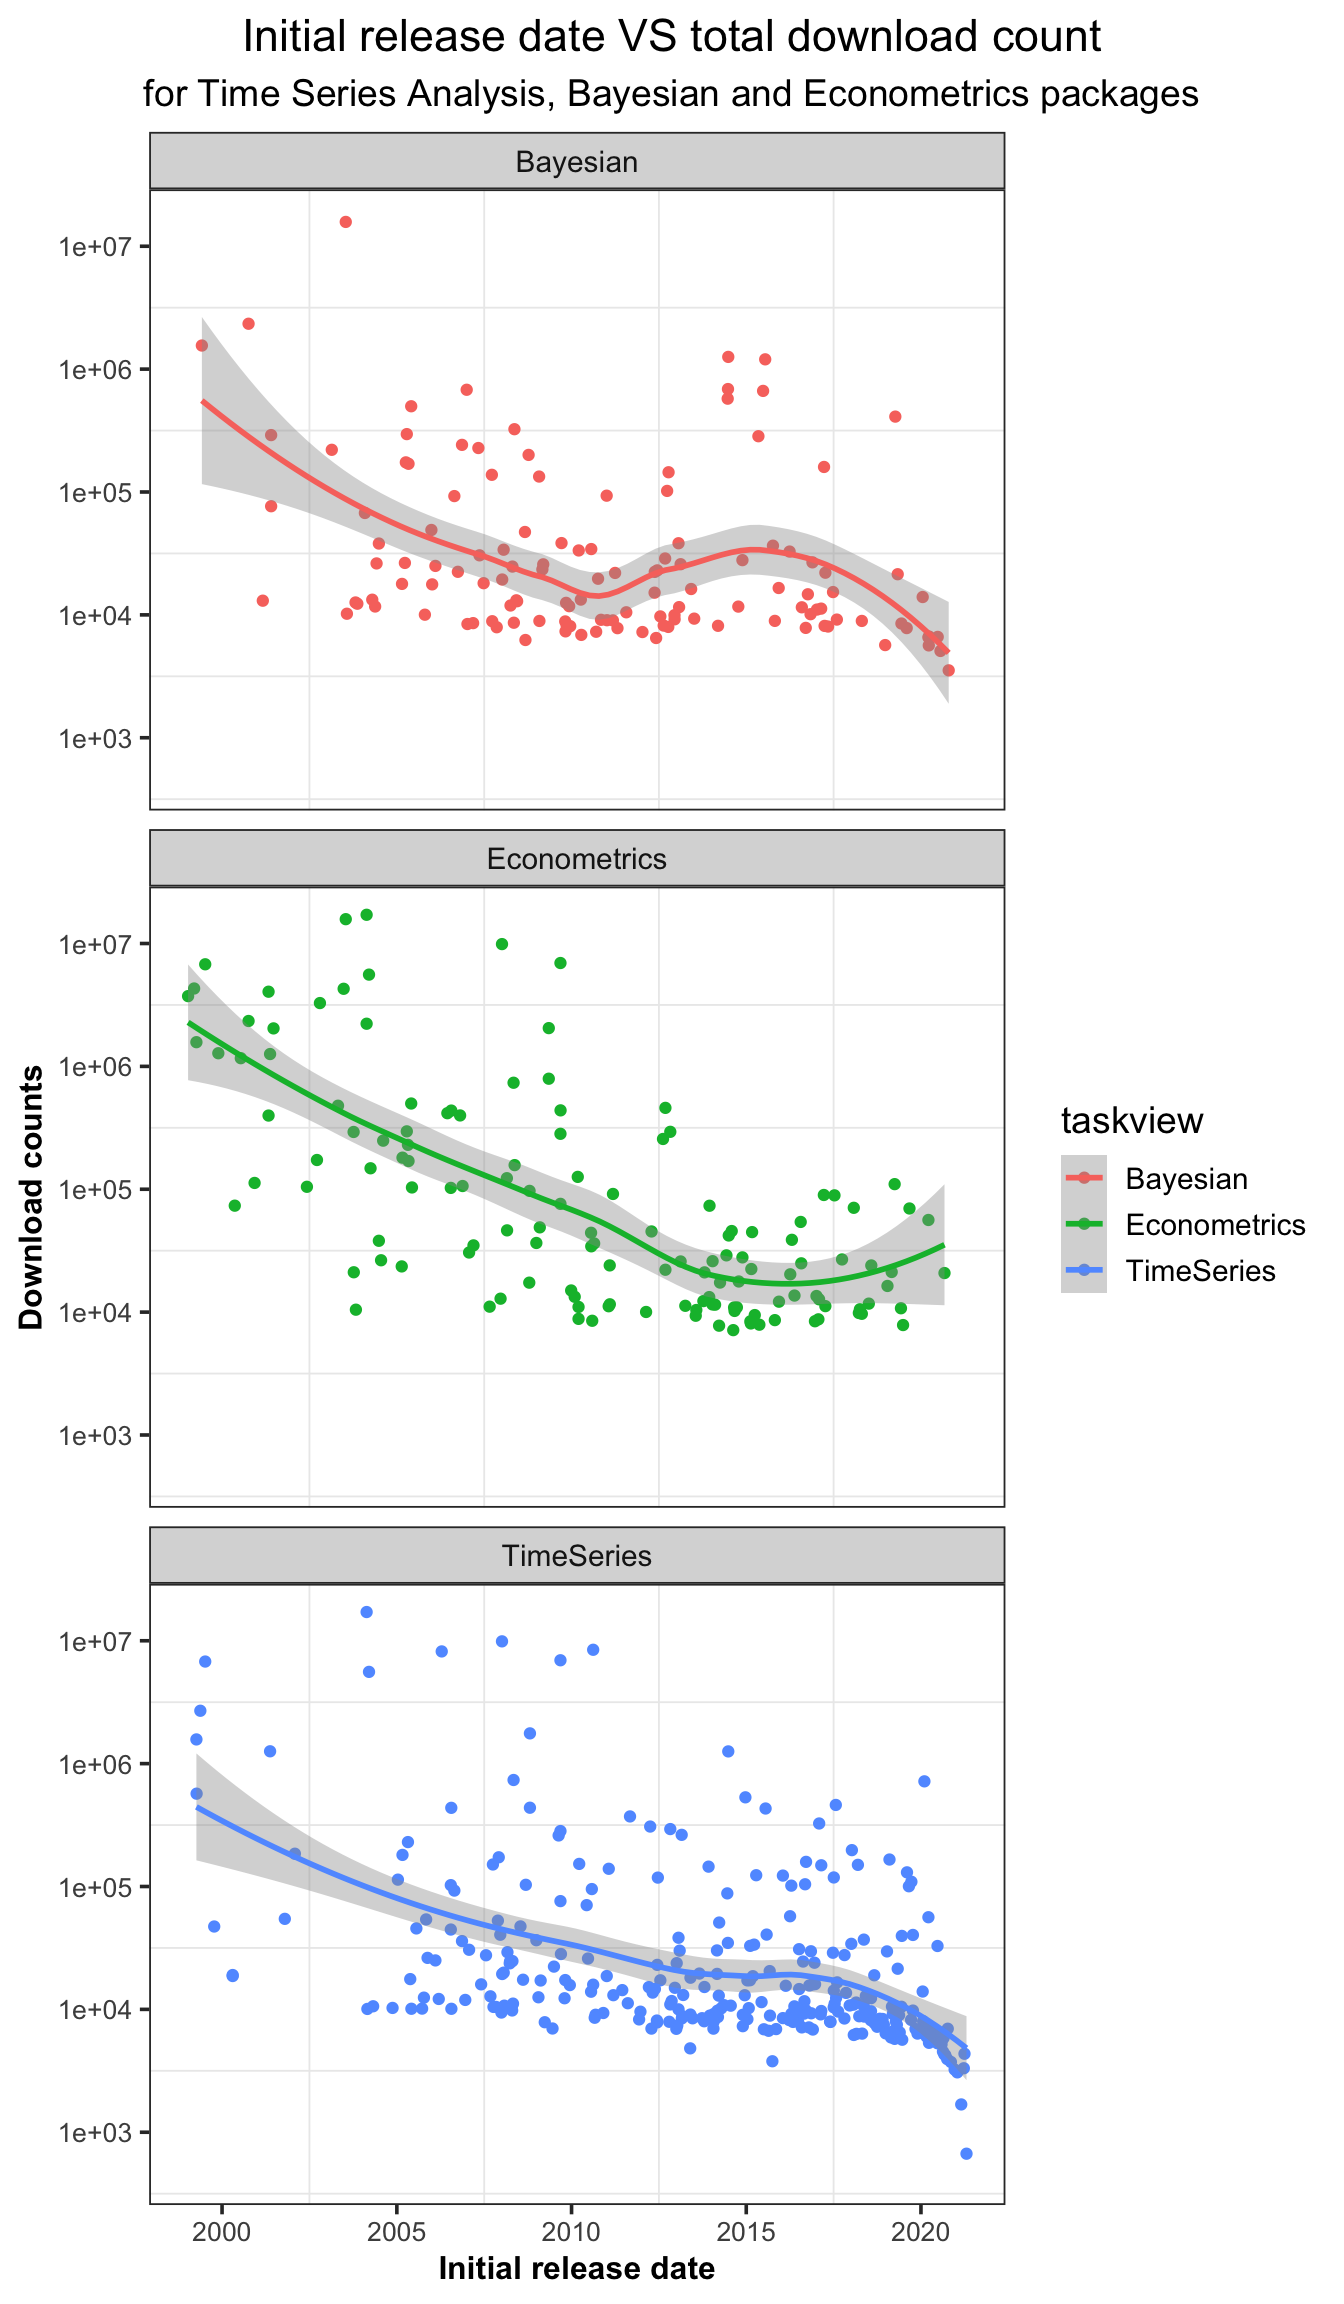
\includegraphics{figures/release-downloads-1} 

}

\caption{The download count decrease with the initial release date.}\label{fig:release-downloads}
\end{figure}

In conclusion, we are not surprised to find that the earlier the R-package is released, the more downloads it could has, which is reflected in all of three topics of R-packages above. That is probably because the R-packages released earlier will be better known. When they are released early, there may be a relatively small number of R-packages of the same topic, under non-serious competition. As a result, the R-packages coming later can easily be covered up, since people generally tend to use well-known, mature and habitual packages.

That is to say, earlier R-packages are more conducive to the cultivation of user habits. After all, habits are influenced by the length of time. For example, if the teacher is an old user of some R-packages, they may recommend these R-packages to their students when they teach, or colleagues may prefer to recommend familiar R-packages to others especially when they get a satisfying user experience.

\hypertarget{compare-moving-average-of-fable-and-forecast}{%
\section{Compare moving average of fable and forecast}\label{compare-moving-average-of-fable-and-forecast}}

\begin{discovery}
\textbf{Finding}: R-package `forecast' has a more stable download trend
comparing to `fable'. And when `fable' gets updated, its downloads
peaked, while `forecast' suffers a dropping on the contrast.
\end{discovery}

As we stated in the previous section, the earlier the R-package is released, the easier it is to get a relatively higher total download. But that doesn't mean a better growth will exist. Due to that, in this section, we compared package \texttt{fable} and \texttt{forecast}. They are two closely related R-packages, for \texttt{fable} is the later released tidy version of \texttt{forecast}. And in this way, we can approximately fix all the factors except the initial release date, so that we can compare the growth and changes of these two more clearly.

Figure \ref{fig:daily-fbl} and Figure \ref{fig:daily-fcst} show the daily download count changing during last half a year, which indicates strong weekly seasonality. And that means the downloads tend to be higher in week days and thus lower on weekends, which is consistent with total R-package trend analyzed before.



\begin{figure}

{\centering 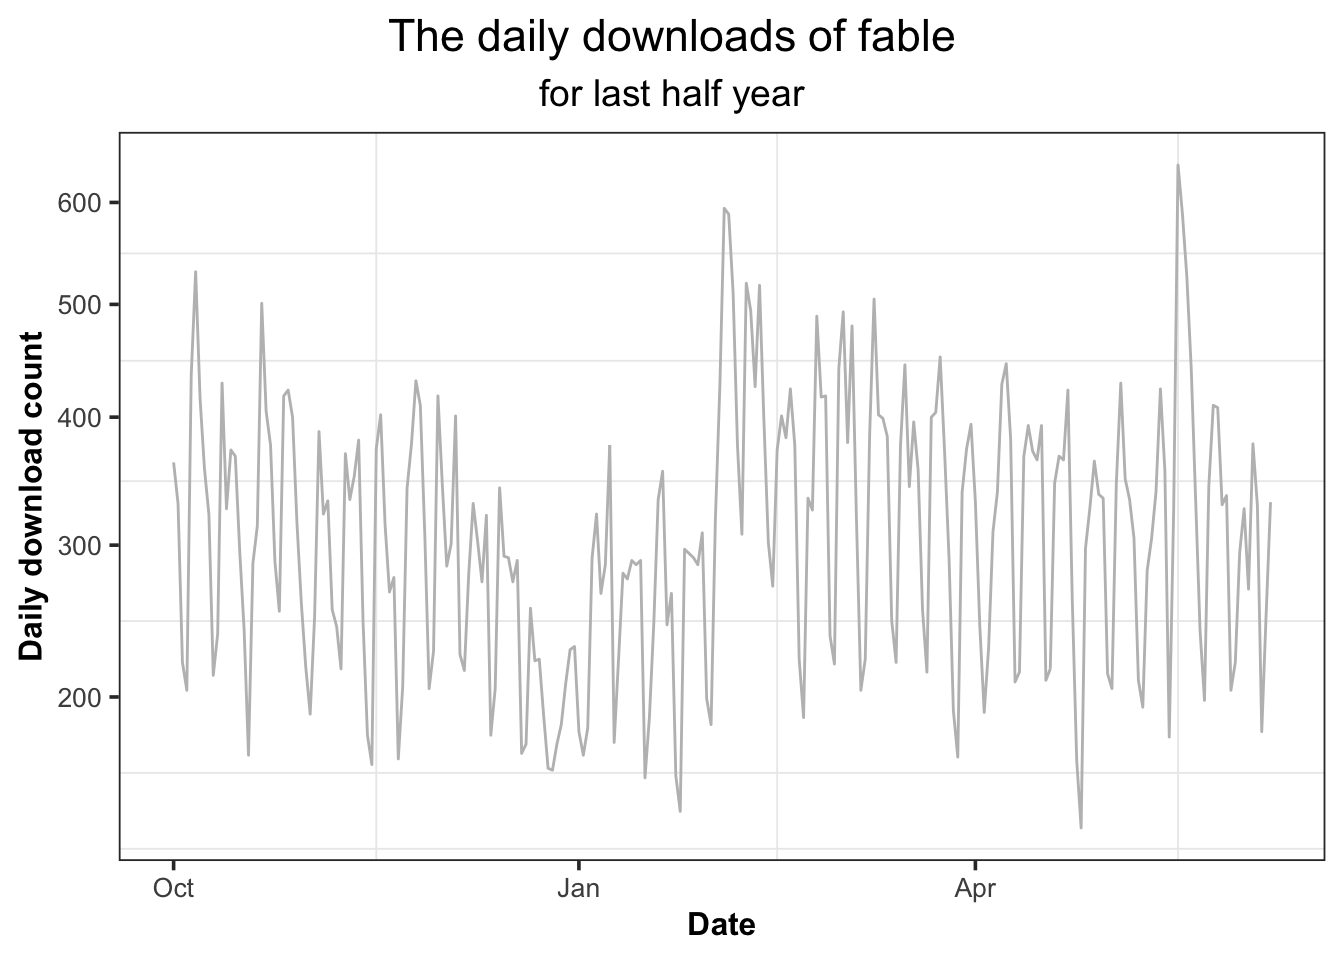
\includegraphics{figures/daily-fbl-1} 

}

\caption{The daily download of R-package ``fable''}\label{fig:daily-fbl}
\end{figure}



\begin{figure}

{\centering 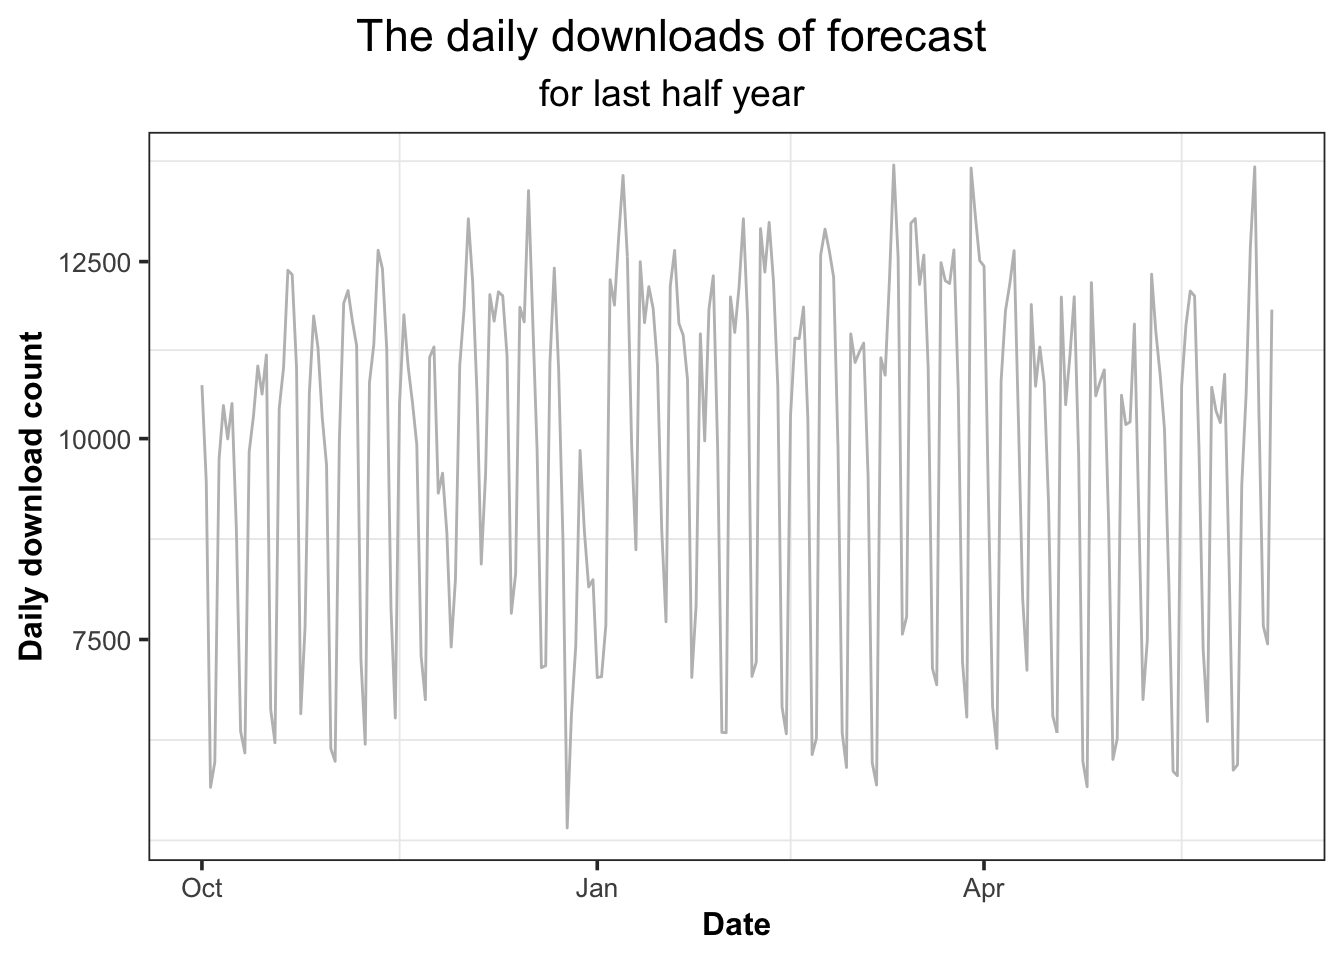
\includegraphics{figures/daily-fcst-1} 

}

\caption{The daily download of R-package ``forecast''.}\label{fig:daily-fcst}
\end{figure}

Therefore, in order to estimate the trend-cycle and reduce the weekly seasonality to see the changes more clearly, we introduced the Moving Average (MA).

A moving average of order \textbf{m} can be written as :

\[T_t = \frac1m\ \Sigma_{j = -k}^{k}y_{t+j} \]

where \textbf{m=2k+1}. That is, the estimate of the trend-cycle at time \textbf{t} is obtained by averaging values of the time series within \textbf{k} periods of \textbf{t}.

And here, we considered the equal weighed 7 moving average. That is, it calculates the weighted average for every seven consecutive time series with the following weights : \emph{{[}1/7,1/7,1/7,1/7,1/7,1/7,1/7{]}}.

Figure \ref{fig:ff-ma} shows the moving average (MA) of \texttt{fable} and \texttt{forecast} respectively. They have quite different moving average patterns with \texttt{forecast}'s download volume much higher than \texttt{fable}'s. That is, the MA of \texttt{forecast} is relatively stable than that of \texttt{fable} except for the time around New Year's Eve when \texttt{forecast} has a significant drop. But during that time, a drop also appears in \texttt{fable}, which was probably due to the big New Year holiday. In addition, the purple vertical dashed line in plot of \texttt{fable} marks the update day of it which is on 2021-1-29. And soon after that day, its downloads peaked, which was because the number of download counts will increase on the update day. At the same time, \texttt{forecast} drops and then only gets a gentle increase.



\begin{figure}

{\centering 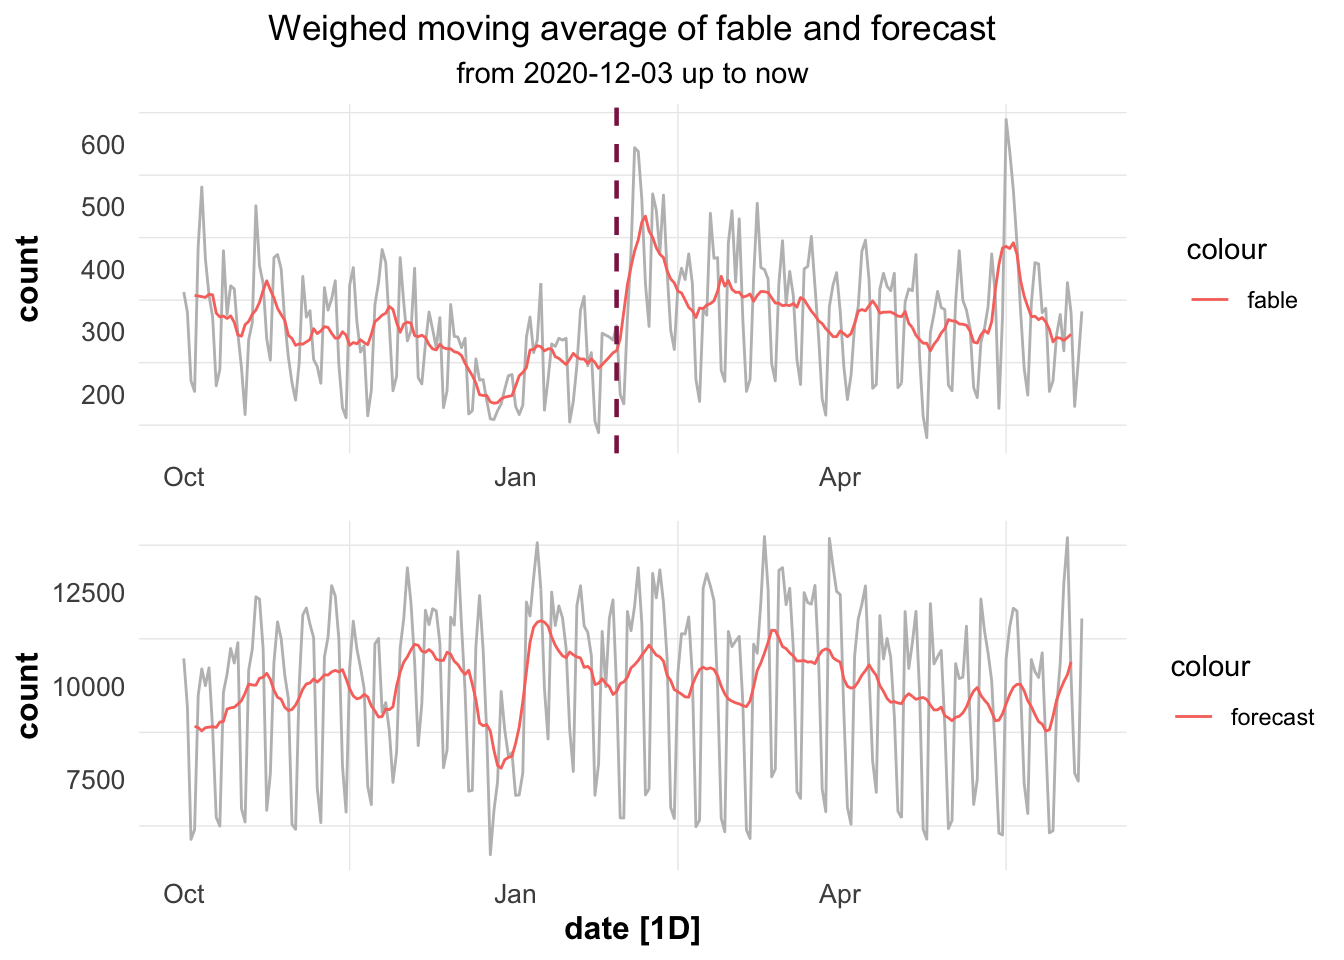
\includegraphics{figures/ff-ma-1} 

}

\caption{The moving average of R-package ``forecast'' and ``fable''.}\label{fig:ff-ma}
\end{figure}

In conclusion, the download variance of \texttt{forecast} is larger than that of \texttt{fable} while the former looks relatively more stable than the latter after applying the moving average. And once again, it coincides with the conclusion of the previous section, that is, the earlier released R-package tends to gain more cumulative downloads. In addition, we can also see that the growth of both of them sometimes increases at the same time, while sometimes the growth of one corresponds to the decline of the other. As for as we concerned, the shared growth may be due to their similarity. Users may download both at the same time or compare them like us. And the trade-off may also be due to the similarity of their functions, one can be replaced by the other in the process of using. Finally, we can also know that earlier release does not guarantee a faster growth. For example, \texttt{fable} has a more dramatic growth than \texttt{forecast} from 2021-01-21 to 2021-02-06.

\hypertarget{compare-download-counts-with-the-number-of-commits-on-master-branch}{%
\section{Compare download counts with the number of commits on master branch}\label{compare-download-counts-with-the-number-of-commits-on-master-branch}}

In this section, we compared last half a year's total downloads with the number of commits on master branch in Github repositories. And this turn, we initially planned to replace the research object with all the R-packages on CRAN, 17,699 up to now. But we soon found out that there were only 6185 R-packages that have a Github repository, and after cleaning up, only 5769 remained.

\begin{discovery}
\textbf{Finding}: In our initial assumption, more commits on master
branch of Github repository tends to bring more download counts to
R-packages. On the one hand, the number of commits indicates that
developers are constantly supplementing and updating the R-package,
which will lead to more downloads. On the other hand, the number of
commits also reflects the attention developers attach to the R-package
to a certain extent. So, if an R-package has more commits, then
developers may invest more in advertising and other ways to promote it,
so as to expand the popularity and improve the download count.
\end{discovery}

The way we initially applied was extracting the commits through accessing the Github API. To achieve this, we first scraped the Github URLs from `description' page for all the R-packages, and cleaned up the multiple URLs or some other redundant symbols and characters. And the URL of scraping the commits through Github API is formatted as \emph{``\url{https://api.github.com/repos/\%7Buser_repo\%7D/commits?per_page=1}''}. For example, the URL for package \texttt{tidyverse} can be like \emph{``\url{https://api.github.com/repos/tidyverse/tidyverse/commits?per_page=1}''}. So, practically, by replacing the \texttt{user\_repo} part that consists of the name of the related repository and the name of the package holder, we could access the content of all the package URLs through Github API.

Based on that, Table \ref{tab:userrepo-tbl} shows the first 5 R-packages of the whole, their Github URLs and the \texttt{user\_repo} part.

However, the Github API has a rate limits allowing for up to 60 requests per hour for unauthenticated requests, and this can be extended to 5000 per hour after authentication\autocite{githubapi}. But even after getting authentication, our rate limit didn't get promoted. So, we switched to scrape commits by python spider. And by setting random user agent, we successfully avoided the API limit. And as this method is quite time consuming (around 5 hours), we saved the output as a .txt file then load it in R studio to speed up the compiling process.

\textbackslash begin\{table\}

\textbackslash caption\{\label{tab:userrepo-tbl}First 5 R-packages with their `user\_repo' element\}
\centering

\begin{tabular}[t]{l|l|l}
\hline
package & URL & user\_repo\\
\hline
abbyyR & http://github.com/soodoku/abbyyR & soodoku/abbyyR\\
\hline
ABCoptim & http://github.com/gvegayon/ABCoptim & gvegayon/ABCoptim\\
\hline
abctools & http://github.com/dennisprangle/abctools & dennisprangle/abctools\\
\hline
abdiv & http://github.com/kylebittinger/abdiv & kylebittinger/abdiv\\
\hline
abess & http://github.com/abess-team/abess & abess-team/abess\\
\hline
\end{tabular}

\textbackslash end\{table\}

Table \ref{tab:commits-tbl} shows the first 5 R-packages of all, along with their last half a year's total downloads and the number of commits on Github master branch.

\begin{table}

\caption{\label{tab:commits-tbl}First 5 R-packages with commits on Github and last half year's total downloads}
\centering
\begin{tabular}[t]{l|l|r}
\hline
package & commits & total\\
\hline
rlang & 4,427 & 14748569\\
\hline
dplyr & 7150 & 12054840\\
\hline
ggplot2 & 4,756 & 11825489\\
\hline
lifecycle & 206 & 10438007\\
\hline
tibble & 4,286 & 10340887\\
\hline
\end{tabular}
\end{table}

Figure \ref{fig:commits-pattern} shows the scatterplot along with a smoothing line. In general, more commits, more downloads.



\begin{figure}

{\centering 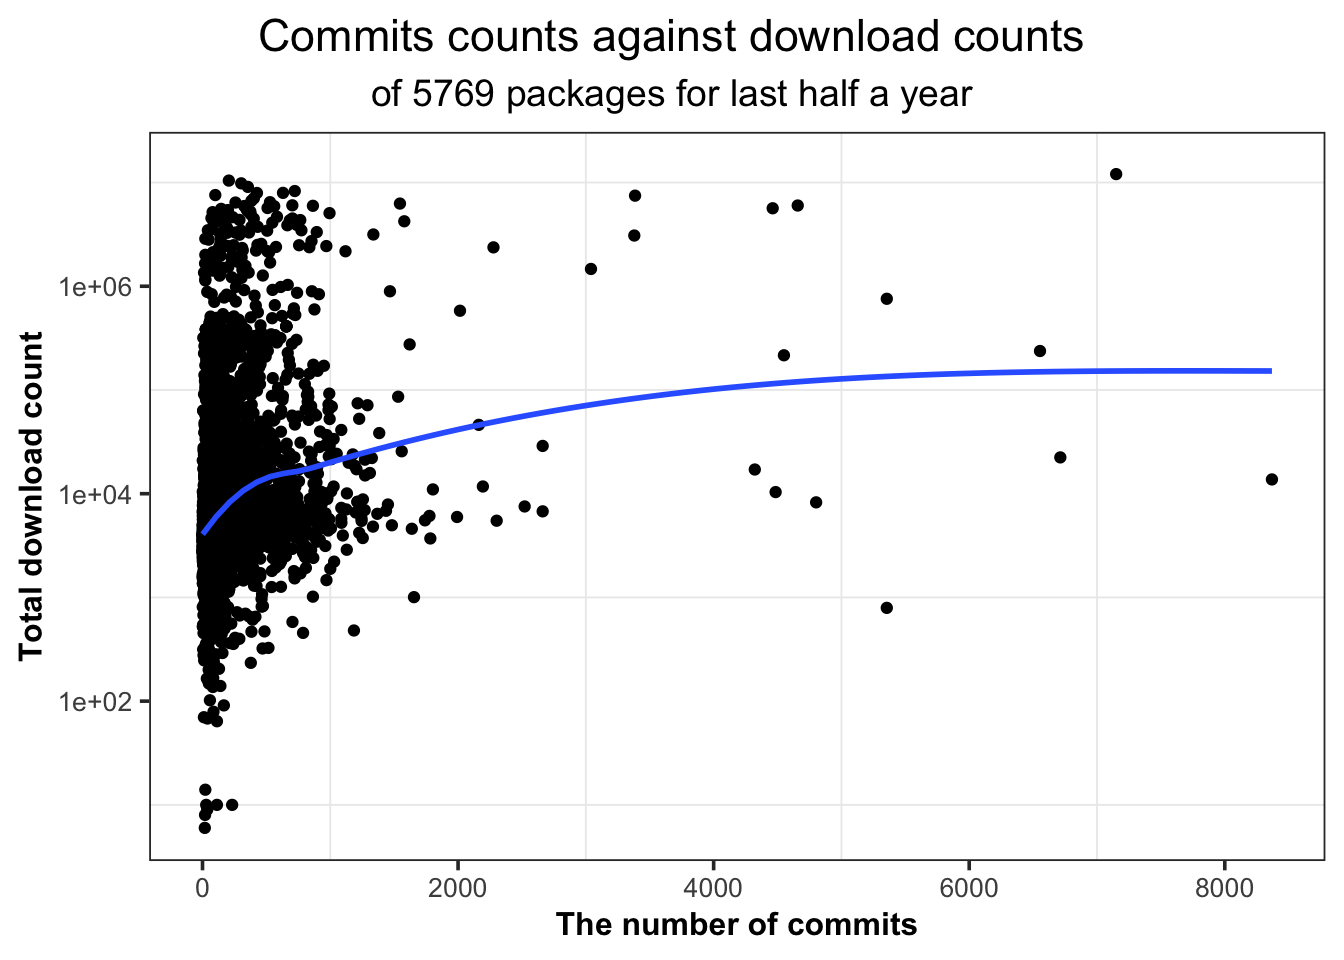
\includegraphics{figures/commits-pattern-1} 

}

\caption{The commits on master branch of Github repository against the last half a year's total download count.}\label{fig:commits-pattern}
\end{figure}

Another method to explore this question is by looking at the ultra-low-downloaded R-packages, whose download count only ranks at last 1\% of all. And another purpose for this part is to show how we initially intended to scrape commits through Github API with R (as the sample size is less than 60 R-packages under this situation).

From Table \ref{tab:quantileall} we could see the last 1\% downloaded count is around 401. And as these download counts are extremely low, we could assume that many factors will have little effect on their downloads. Thus, we can further assume that the only two differences between them are the number of commits on Github master branch and the total download count.

So, we could filter these ultra-low-downloaded R-packages and extract the commits on Github, then explore the pattern in total download count against the number of commits in Figure \ref{fig:pkg-low}. It could be believed that when the number of commits increases from 0 to 100, the download count first increases and then decreases. After that, the download volume keeps rising and appears to have a little jump at the end, but we supposed it might be due to the the too small-sized sample, and the observation causing the decline may be an outlier. So, if expanding the observation horizon, we expected the curve might increase again. Therefore, it can be seen that even for these last 1\% downloaded R-packages, there also exist the phenomenon - ``the more commits, the more downloads''.

\begin{table}

\caption{\label{tab:quantileall}Quantile of total download count for all the R-packages on CRAN}
\centering
\begin{tabular}[t]{l|r}
\hline
  & download count\\
\hline
0\% & 0.00\\
\hline
1\% & 373.00\\
\hline
2\% & 716.00\\
\hline
3\% & 1087.65\\
\hline
4\% & 1365.20\\
\hline
5\% & 1667.50\\
\hline
6\% & 1915.30\\
\hline
7\% & 2185.85\\
\hline
8\% & 2334.00\\
\hline
9\% & 2512.00\\
\hline
10\% & 2686.50\\
\hline
11\% & 2796.00\\
\hline
12\% & 2862.60\\
\hline
13\% & 2913.00\\
\hline
14\% & 2967.00\\
\hline
15\% & 3027.00\\
\hline
16\% & 3087.00\\
\hline
17\% & 3156.00\\
\hline
18\% & 3245.00\\
\hline
19\% & 3333.00\\
\hline
20\% & 3406.00\\
\hline
21\% & 3466.00\\
\hline
22\% & 3532.00\\
\hline
23\% & 3581.00\\
\hline
24\% & 3627.00\\
\hline
25\% & 3664.00\\
\hline
26\% & 3700.00\\
\hline
27\% & 3731.85\\
\hline
28\% & 3766.00\\
\hline
29\% & 3808.00\\
\hline
30\% & 3846.00\\
\hline
31\% & 3884.00\\
\hline
32\% & 3929.00\\
\hline
33\% & 3973.15\\
\hline
34\% & 4016.00\\
\hline
35\% & 4062.00\\
\hline
36\% & 4101.00\\
\hline
37\% & 4141.00\\
\hline
38\% & 4187.00\\
\hline
39\% & 4227.00\\
\hline
40\% & 4269.00\\
\hline
41\% & 4310.00\\
\hline
42\% & 4352.00\\
\hline
43\% & 4391.00\\
\hline
44\% & 4434.20\\
\hline
45\% & 4477.75\\
\hline
46\% & 4527.00\\
\hline
47\% & 4568.00\\
\hline
48\% & 4617.00\\
\hline
49\% & 4659.00\\
\hline
50\% & 4703.00\\
\hline
51\% & 4745.00\\
\hline
52\% & 4785.00\\
\hline
53\% & 4829.00\\
\hline
54\% & 4880.00\\
\hline
55\% & 4931.00\\
\hline
56\% & 4983.80\\
\hline
57\% & 5048.00\\
\hline
58\% & 5103.00\\
\hline
59\% & 5167.00\\
\hline
60\% & 5233.00\\
\hline
61\% & 5293.00\\
\hline
62\% & 5356.00\\
\hline
63\% & 5410.65\\
\hline
64\% & 5470.00\\
\hline
65\% & 5543.00\\
\hline
66\% & 5610.30\\
\hline
67\% & 5693.00\\
\hline
68\% & 5774.00\\
\hline
69\% & 5863.00\\
\hline
70\% & 5965.00\\
\hline
71\% & 6085.05\\
\hline
72\% & 6232.00\\
\hline
73\% & 6395.00\\
\hline
74\% & 6581.00\\
\hline
75\% & 6772.00\\
\hline
76\% & 6987.00\\
\hline
77\% & 7229.75\\
\hline
78\% & 7530.80\\
\hline
79\% & 7889.15\\
\hline
80\% & 8313.00\\
\hline
81\% & 8757.65\\
\hline
82\% & 9438.10\\
\hline
83\% & 10246.60\\
\hline
84\% & 11414.00\\
\hline
85\% & 12868.75\\
\hline
86\% & 14534.30\\
\hline
87\% & 16524.85\\
\hline
88\% & 18997.40\\
\hline
89\% & 21799.10\\
\hline
90\% & 25522.50\\
\hline
91\% & 30952.45\\
\hline
92\% & 39941.00\\
\hline
93\% & 52296.65\\
\hline
94\% & 69259.80\\
\hline
95\% & 100932.00\\
\hline
96\% & 150491.20\\
\hline
97\% & 255838.40\\
\hline
98\% & 477013.80\\
\hline
99\% & 1909210.00\\
\hline
100\% & 15572507.00\\
\hline
\end{tabular}
\end{table}



\begin{figure}

{\centering 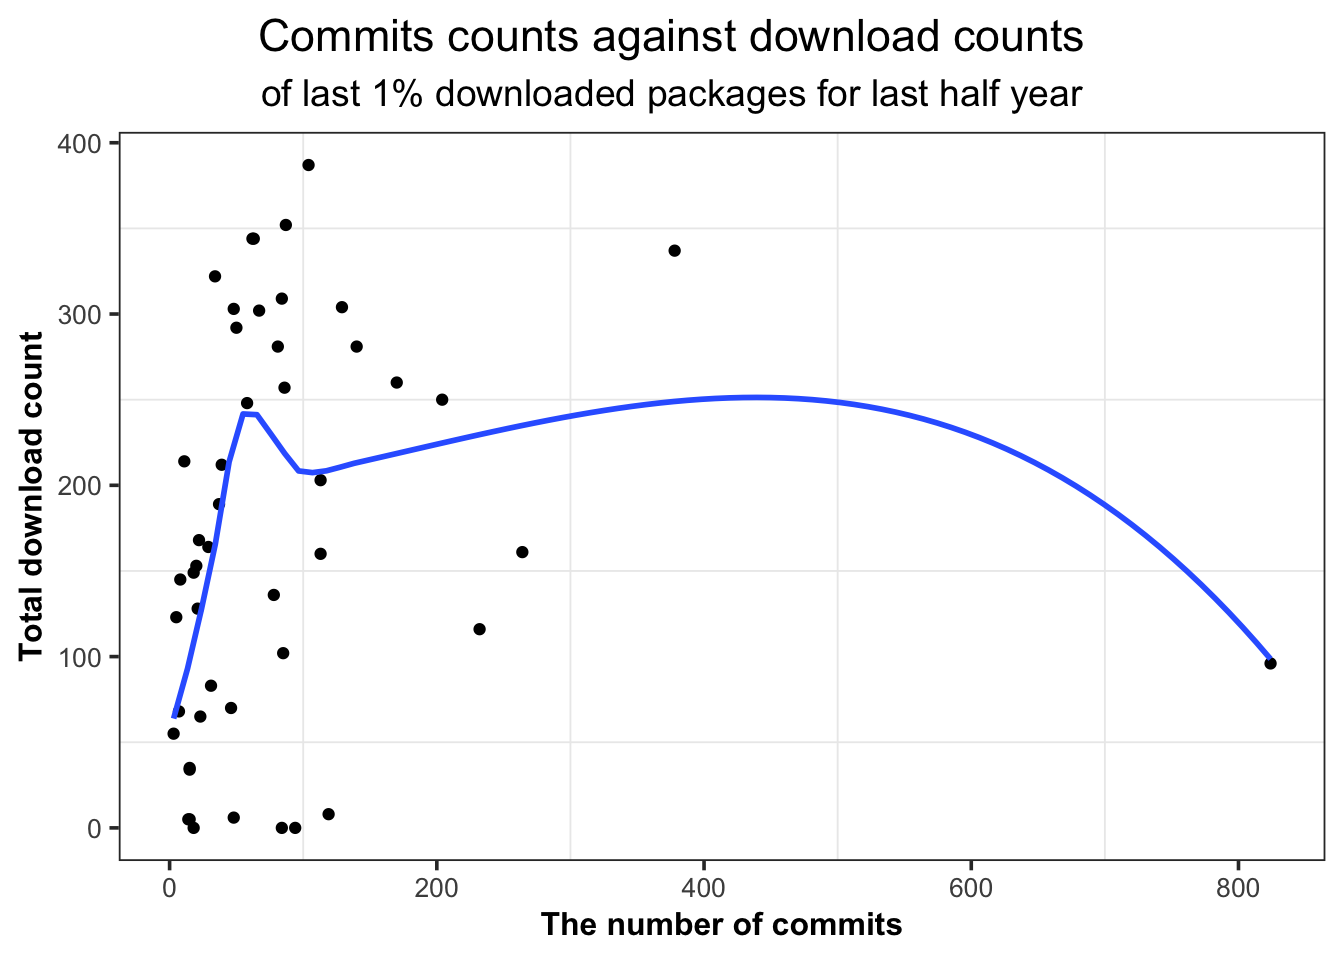
\includegraphics{figures/pkg-low-1} 

}

\caption{The commits on master branch of Github repository against the last half a year's total download count for last 1\% downloaded R-packages on CRAN.}\label{fig:pkg-low}
\end{figure}

\hypertarget{compare-download-counts-with-the-number-of-updates}{%
\section{Compare download counts with the number of updates}\label{compare-download-counts-with-the-number-of-updates}}

Next, let's look at the relationship between the number of updates and the number of downloads.
In this part, our analysis object is still all the packages.

\begin{discovery}
\textbf{Finding 1}: The download count tends to rise with the number of
updates.This is because as we have known before, when a package is
updated, there will be a significant increase in the number of
downloads. That is to say, when a package is updated, not only old users
will download the latest version, but also it is easier to attract new
users at this time, for the increase of downloads in a short time may
bring it into the trending list.
\end{discovery}

Figure \ref{fig:all-updates} shows that the number of downloads increases with the update times. And most R-packages are updated no more than 30 times.



\begin{figure}

{\centering 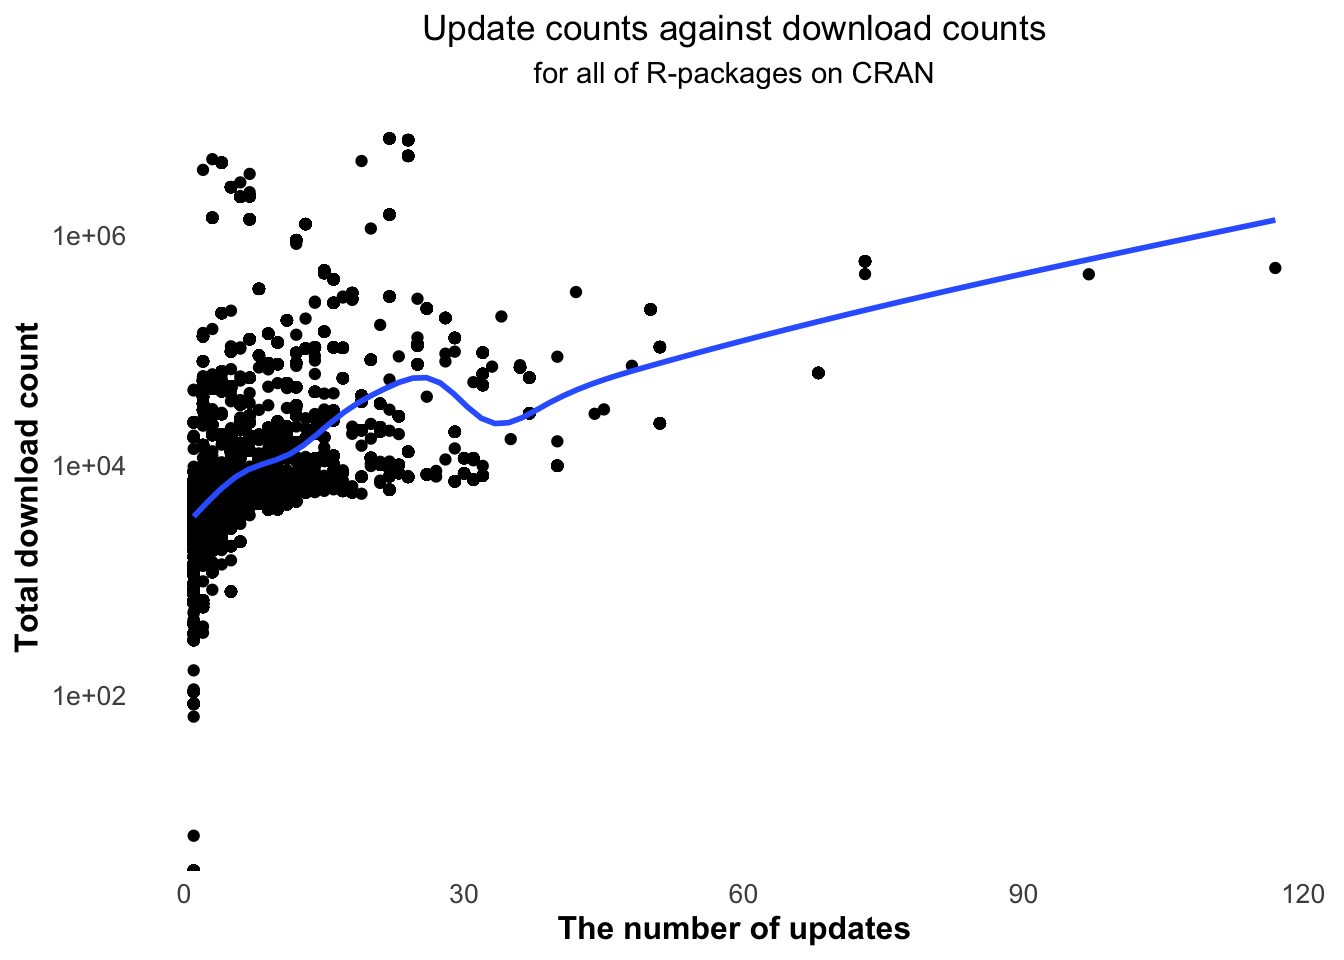
\includegraphics{figures/all-updates-1} 

}

\caption{The download count increase with the number of updates.}\label{fig:all-updates}
\end{figure}

\begin{discovery}
\textbf{Finding 2}: Over half of the R-packages don't tend to update
very frequently.
\end{discovery}

Also checking Table \ref{tab:pct-lowupdates}, we can know that the percentage of R-packages whose updates are less than average is 70.2920266 \%, which means much more than half of the R-packages do not tend to update very frequently.

\begin{table}

\caption{\label{tab:pct-lowupdates}Percentage of trending R-packages whose updates are less than average}
\centering
\begin{tabular}[t]{r|r}
\hline
number of packages with low updates & percentage of packages with low updates\\
\hline
11963 & 70.29203\\
\hline
\end{tabular}
\end{table}

\begin{discovery}
\textbf{Finding 3}: Most R-packages keep updating with the time to keep
its activity.
\end{discovery}

It can be seen from Figure \ref{fig:latestpublish} that most R-packages' latest publish date is after 2015, which indicates that many R-packages tend to update by time to keep its activity.



\begin{figure}

{\centering 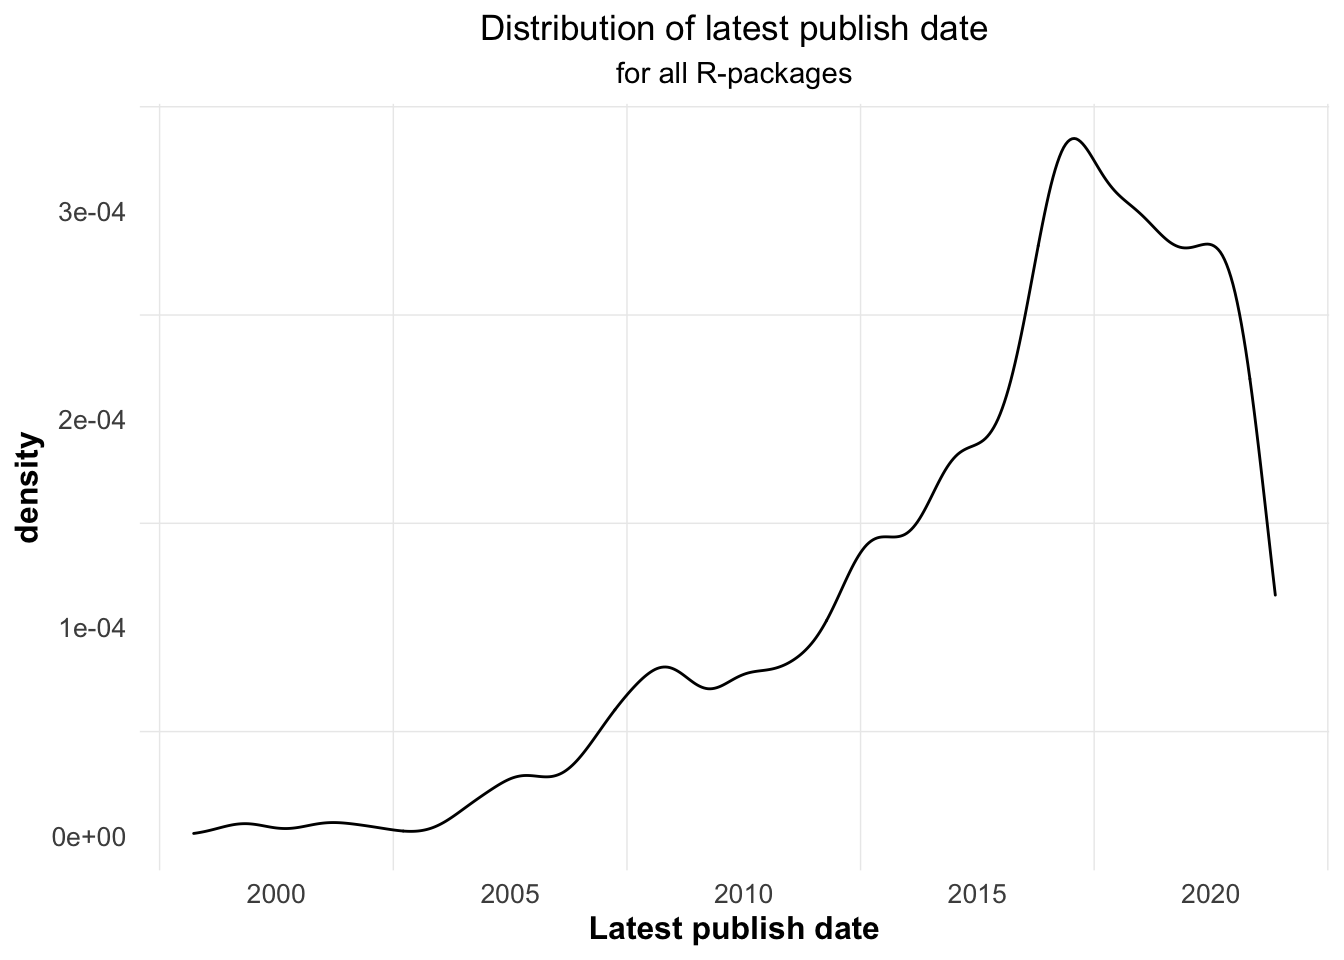
\includegraphics{figures/latestpublish-1} 

}

\caption{The latest update dates of trending R-packages are almost all the recent dates.}\label{fig:latestpublish}
\end{figure}

\begin{discovery}
\textbf{Finding 4}: Most of the R-packages are likely to update at a
longer time interval.
\end{discovery}

Figure \ref{fig:updates-perday} shows that with the increase of update interval, the number of downloads first increases and then decreases slightly. And most of the time intervals are between 45 and 450 days, which shows that their update frequency is not very high.



\begin{figure}

{\centering 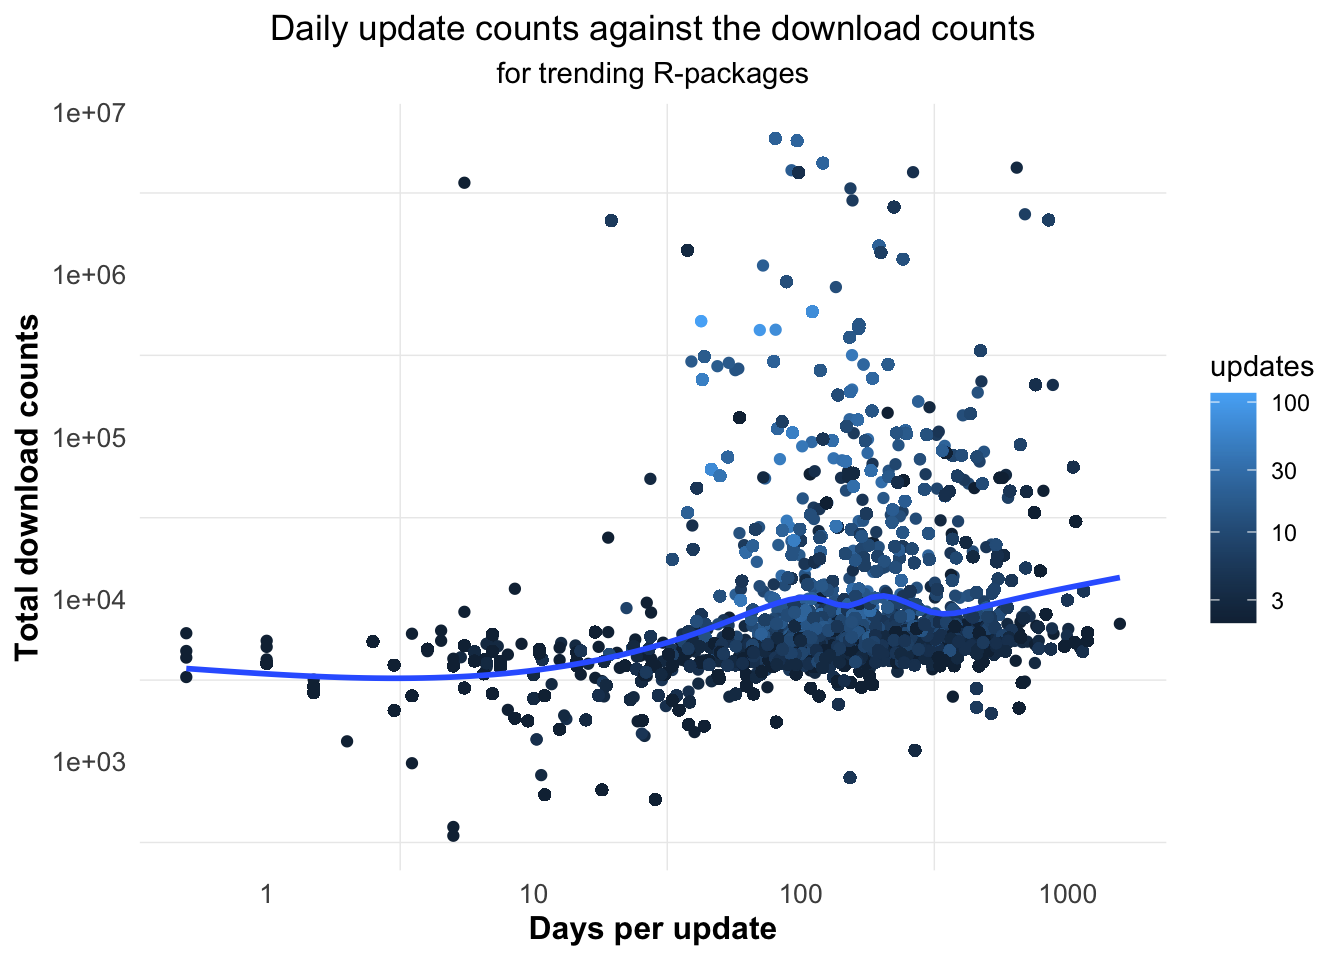
\includegraphics{figures/updates-perday-1} 

}

\caption{Most of the time intervals of updates are between 45 and 450 days.}\label{fig:updates-perday}
\end{figure}

In conclusion, it's not that the more updates the R-package has, the popular it will be. In general, most of the R-packages whose updates are lower than the average occupy the majority. Therefore, we can also know that the total number of updates is not very important for the R-package. The important thing is to keep it updated with the time.

\hypertarget{compare-the-package-name-length-with-download-counts}{%
\section{Compare the package name length with download counts}\label{compare-the-package-name-length-with-download-counts}}

Here, we still focused on all R-packages on CRAN and made comparison between the name length with the last half a year's total downloads.

\begin{discovery}
\textbf{Finding 1}: The name length of R-packages has no significant
effect on the number of total downloads for last half a year.
\end{discovery}

We could see from Figure \ref{fig:namelength-plot} that, in general, the influence of name length on download volume is not very obvious. But we could still observe that the number of downloads decreases slightly with the length of the name. And the names with more than 6,000,000 downloads are between 5 and 9 characters long. Also, the most downloaded is R-package rlang whose name length is 5, with \ensuremath{1.5572507\times 10^{7}} download counts.



\begin{figure}

{\centering 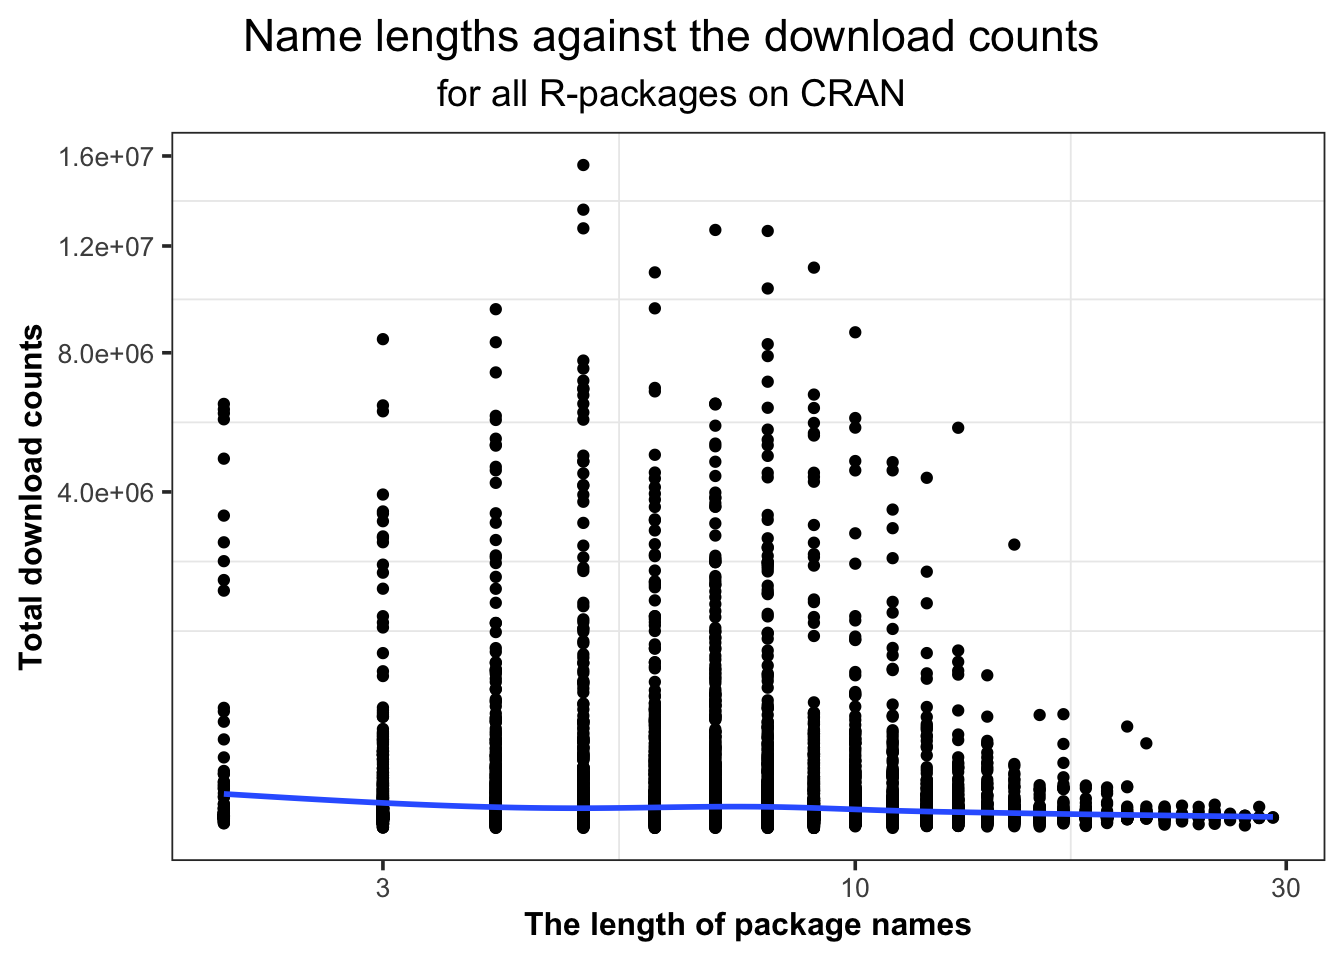
\includegraphics{figures/namelength-plot-1} 

}

\caption{The names of R-packages with more than 6,000,000 downloads are between 5 and 9 characters long.}\label{fig:namelength-plot}
\end{figure}

\begin{discovery}
\textbf{Finding 2}: The average name length of R-packages is about 7.8
characters, and over half of the R-packages tend to have shorter names,
which may make it more easier to be remembered by users.
\end{discovery}

Table \ref{tab:pct-lngname} shows that the average name length all R-packages is 7.8461146. And over half of the R-packages are more likely to have names shorter than average. That means, to a certain extent, R-packages with shorter names are easier to get relatively higher downloads. And that may because shorter named packages are easier for users to remember.

\begin{table}

\caption{\label{tab:pct-lngname}Percentage of packages whose name length are less than average}
\centering
\begin{tabular}[t]{r|r|r}
\hline
number of short names & percentage of short names & total average name length\\
\hline
9286 & 52.59402 & 7.846115\\
\hline
\end{tabular}
\end{table}

\begin{discovery}
\textbf{Finding 3}: The 95\% confidence interval of the name length is
between 7.80 and 7.90 characters.
\end{discovery}

Table \ref{tab:pct-lngname} shows the 95\% confidence interval of name length for all packages. We could know that the 95\% suitable name length is between 7.7936087 and 7.8986206 characters.

\textbackslash begin\{table\}

\textbackslash caption\{\label{tab:namelth-ci}95\% Confidence Interval of name length for random packages\}
\centering

\begin{tabular}[t]{r|r}
\hline
lower.bound & upper.bound\\
\hline
7.793609 & 7.898621\\
\hline
\end{tabular}

\textbackslash end\{table\}

After we found that there is no obvious relationship between the name length of the package and the download volume, a new question came up : Is the name length of the package affected by the time of initial release date?

\begin{discovery}
\textbf{Finding 4}: For taskview R-packages, the length of the package
name increases with the initial release date, especially for Bayesian
packages.
\end{discovery}

We have such an experience in life, that is, for the same type of goods, such as detective novels, the later they are released, the narrower the choice of naming is, because there are certain restrictions on the name of a particular type, but many names have been occupied by the books published earlier. Therefore, these later published books often have to lengthen their names to distinguish themselves from the existing books in the same type or even the same name.
Coincidentally, we assumed the naming of R-packages from the same topic would also be affected by the initial release time, to a certain extent. So, here, we looked back to the CRAN task view R-packages for constructing comparison among R-packages from the same topic. Figure \ref{fig:namelth-taskview} shows the name length of CRAN task view R-packages against the initial release date. It is obvious that the length of the R-package name increases with the initial release date, especially for Bayesian R-packages.



\begin{figure}

{\centering 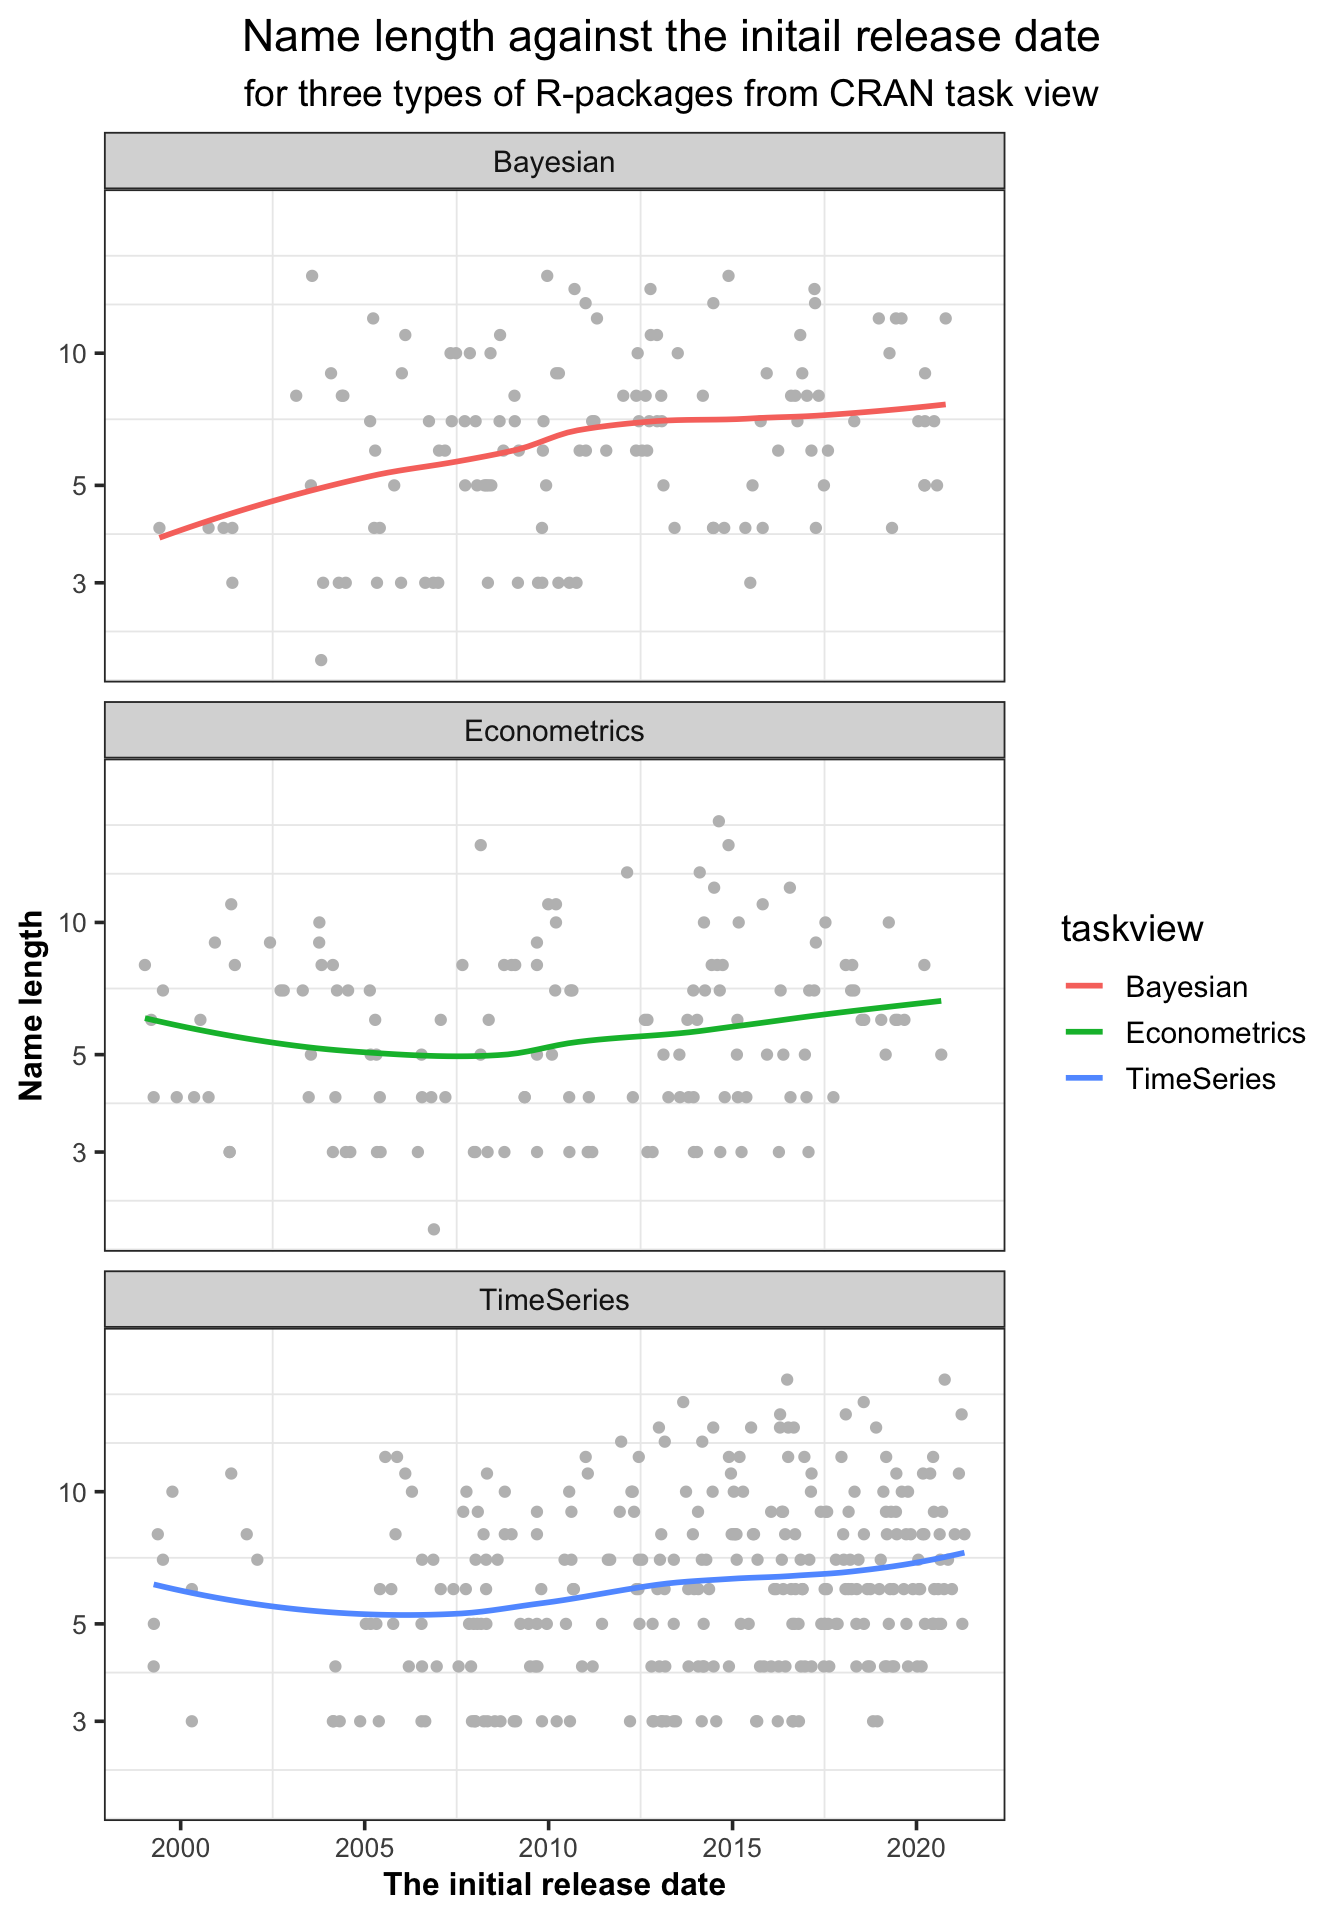
\includegraphics{figures/namelth-taskview-1} 

}

\caption{The name length of taskview R-packages slightly increase with the initial release date.}\label{fig:namelth-taskview}
\end{figure}

\begin{discovery}
\textbf{Finding 5}: For all R-packages on CRAN, the average name length
tends to generally increase with the initial release date.
\end{discovery}

Although we'd better explore this question among the same topic of R-packages, we could also have a view on the annual change in the average name length of all R-packages on CRAN.

Figure \ref{fig:avgnamelth-year} shows the average name length of all R-packages on CRAN released in each year. It is obvious that the name length of these R-package generally increases year by year.



\begin{figure}

{\centering 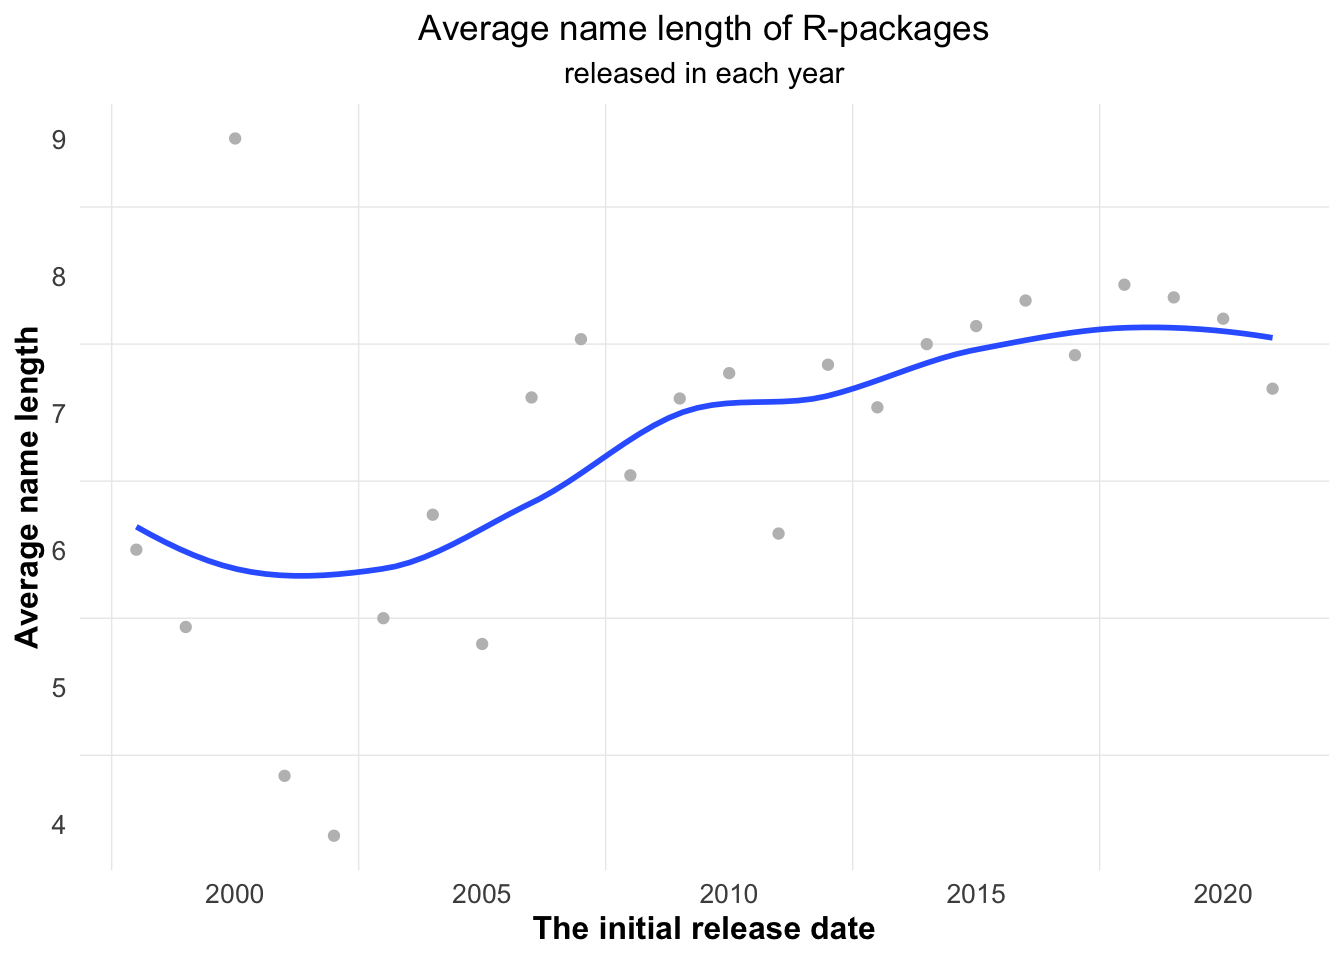
\includegraphics{figures/avgnamelth-year-1} 

}

\caption{(ref:avgnamelth-year)}\label{fig:avgnamelth-year}
\end{figure}

\hypertarget{compare-download-counts-with-alphabetical-order-of-name}{%
\section{Compare download counts with alphabetical order of name}\label{compare-download-counts-with-alphabetical-order-of-name}}

We might also have such experiences in our life. For example, when we go shopping in the supermarket, the goods placed in front of the shelves will be easier to attract our attention and be selected by us, because we may no longer want to seek products with similar functions for a long time.

From the perspective of R-package name, in addition to the length, is the alphabetical order of the first letter also linked the download volume? For R-packages with earlier alphabetical order will be placed at the first part of the R-package list on CRAN\autocite{cranpkgsname}. To answer this question, we grouped the R-packages by 26-letter order, calculated the average downloads of each group, and then made comparison.

\begin{discovery}
\textbf{Finding 1}: For all R-packages, the average downloads of
different alphabetical group are slightly increasing by its order, while
the total download tends to decrease a little, instead.
\end{discovery}

From Figure \ref{fig:ahlpha-downloads} we could see that the average downloads of different alphabetical group are slightly increasing by alphabetical order, while the total downloads tends to decrease a little, instead. This is because the later-ordered group contains fewer R-packages. It can be seen that developers may prefer to name their packages with a top alphabetical order, which might be easier for users to notice.



\begin{figure}

{\centering 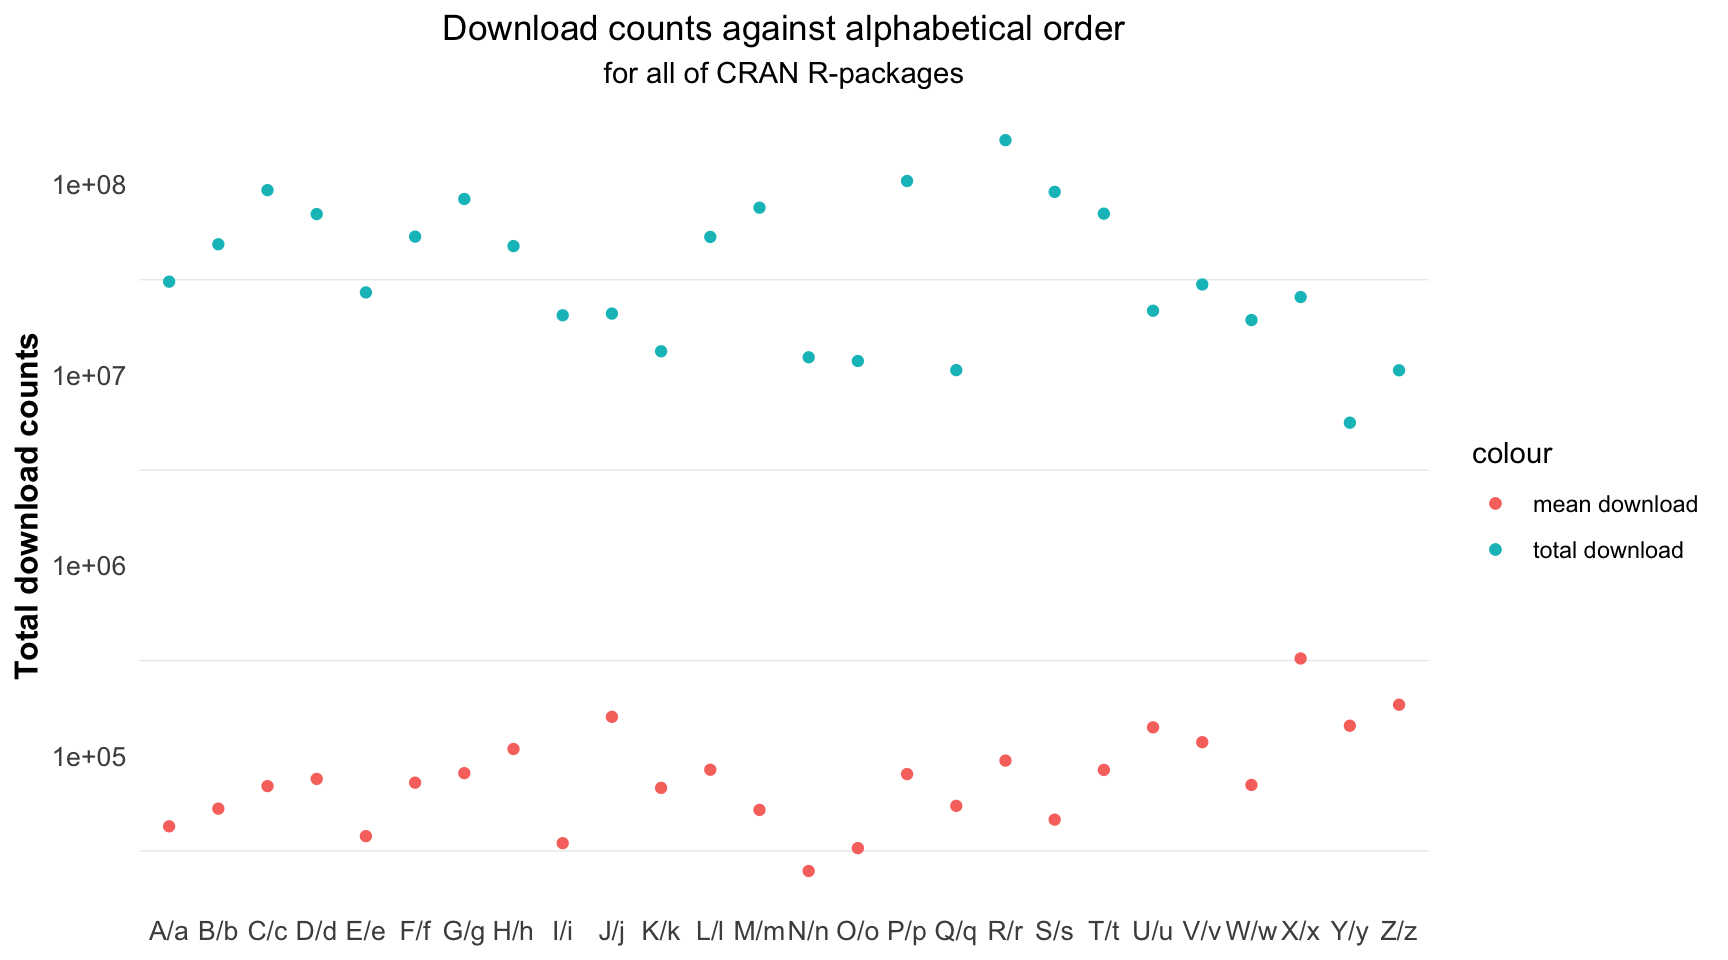
\includegraphics{figures/ahlpha-downloads-1} 

}

\caption{The average total download count of each group is little linked to the alphabetical order of R-package name.}\label{fig:ahlpha-downloads}
\end{figure}

\begin{discovery}
\textbf{Finding 2}: For all R-packages on CRAN, the group with higher
total download tends to have greater variance, owing to more outliers.
\end{discovery}

Then, let's take a look for how the variance varies across groups. Figure \ref{fig:all-boxplot} shows the data range and the median value for each alphabetical group. It can be seen that the group ``R/r'' has the highest outlier and the group ``X/x'' has the largest variation. At the same time, we could also see that the variance between different groups is not very obvious, which means that for each group, 50\% of the R-package download count is relatively concentrated. The real difference is the highest and lowest downloads per group. In general, the larger the total number of downloads (which also means the more packages in the group), the more outliers will be included, such as group ``F/f'', ``L/l'' and ``R/r''.



\begin{figure}

{\centering 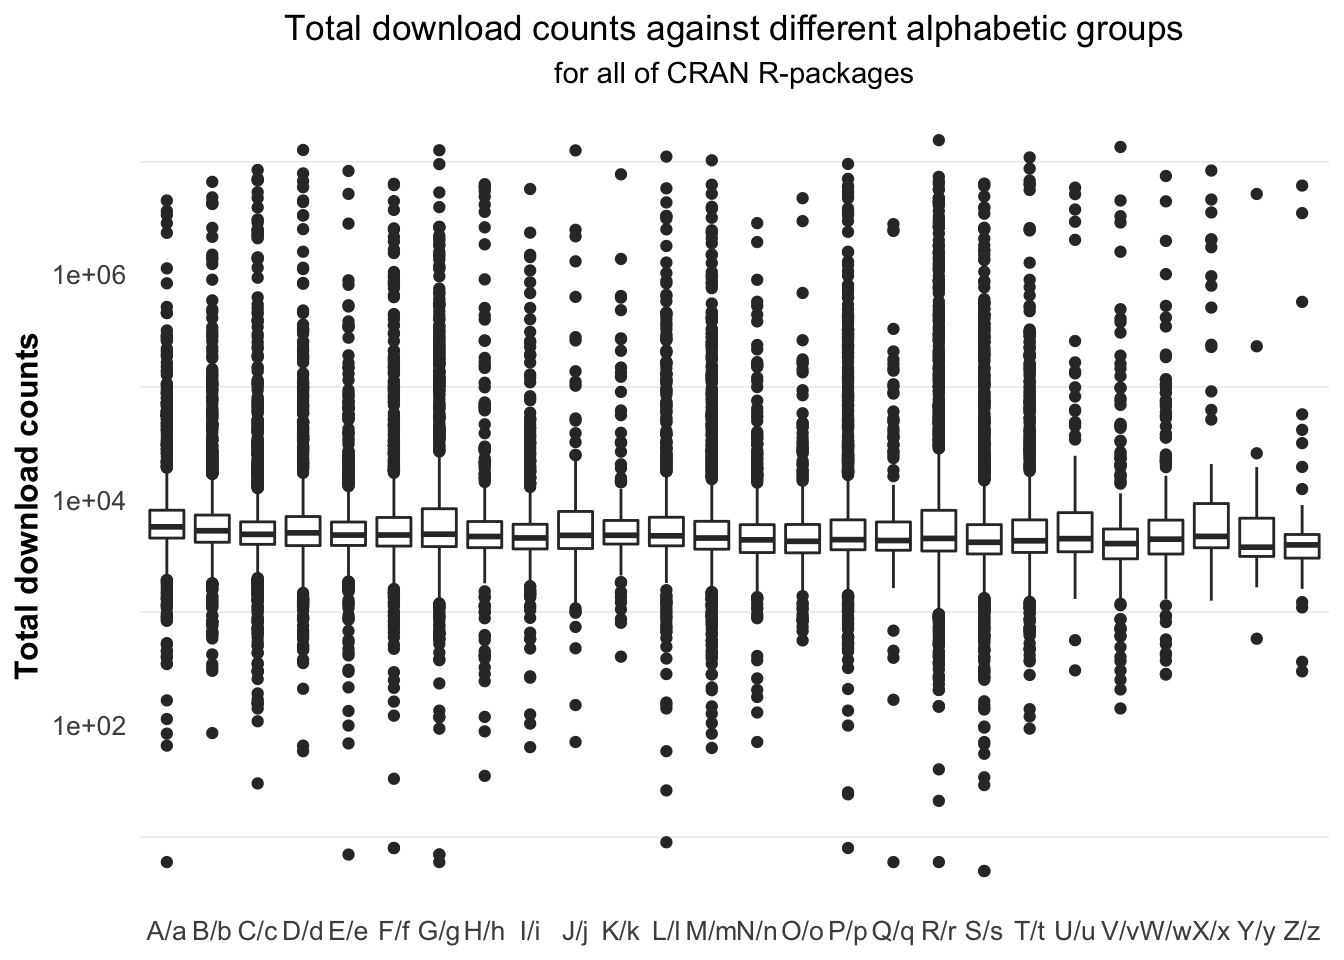
\includegraphics{figures/all-boxplot-1} 

}

\caption{The R-packages with name starting with ``j'' has the largest variation.}\label{fig:all-boxplot}
\end{figure}

In order to further verify our conclusion, we turned to the ultra-low-downloaded R-packages. As we have mentioned previously, when it comes to the ultra-low-downloaded R-packages, we could approximately assume the only variable that may affect the amount of downloads is name order here.
From Figure \ref{fig:lowdownload-boxplot}, we could see that the difference in median download count of each alphabetical group is not significant as we expected.

\begin{figure}

{\centering 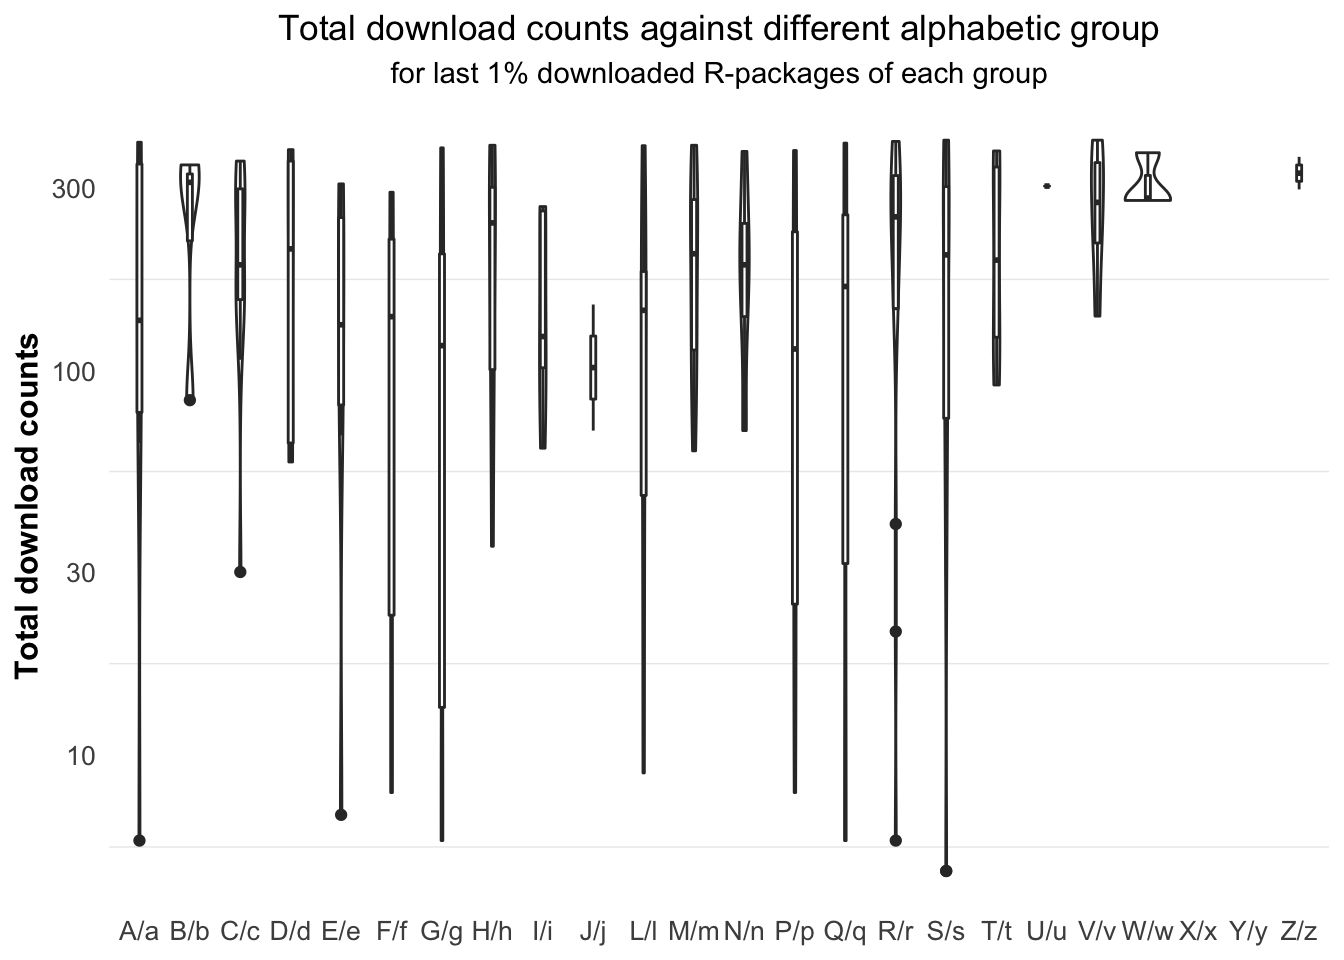
\includegraphics{figures/lowdownload-boxplot-1} 

}

\caption{(ref:random-boxplot)}\label{fig:lowdownload-boxplot}
\end{figure}

Therefore, we could approximately draw a conclusion : In general, the R-packages with the top alphabetical order are easier to get relatively high download volume, but the gap is not significant. At the same time, the higher the number of downloads, the greater the variance will appears in this group.

\hypertarget{summary}{%
\chapter{Summary}\label{summary}}

In this project, we collected summary daily download logs of R-packages through web Application Programming Interface (API) maintained by r-hub\autocite{rhub} and also used daily download data in CRAN for a time period from 2013-04-01 to 2021-04-01 to explore the daily download pattern of all R-packages both in general and of each year. In that case, we found that it is true that the cumulative number of downloads increases with time, and the variance also increases, which indicates that some R-packages with larger downloads grow rapidly. In addition, there is also strong weekly seasonality in the daily download plot. The download count will peak through weekdays and drop on weekend, for users may tend to work and study during weekdays while rest on weekends. What's more, through Lorenz curve, we also found that most of the cumulative downloads came from the top 10\% downloaded R-packages, so we could also see that the distribution of downloads is quite unequal. Part of the reason is that these top 10\% downloaded R-packages contain quite a lot popular and frequently used R-packages, such as \texttt{tidyverse} and \texttt{rlang}, which would be more probably to gain high downloads. In addition, there are other R-packages that often get high download volume, which can be divided into the following four categories:

\begin{itemize}
\tightlist
\item
  R-packages maintained by R studio
\item
  R-packages created by authors from R core group
\item
  R-packages created by authors from R secondary group
\item
  R-packages created by R related authors
\item
  R-packages created by top 20 prolific maintainers (This is resourced at \textcite{revolutions})
\end{itemize}

However, the existence of these R-packages may make it difficult to reflect the popularity of other R-packages, so we excluded these R-packages for the analysis of user preferences. And we found that the topic of newly added R-packages on 1st Oct of each year are from quite different areas, while the R-packages remaining most stably popular during 2017 to 2019 is about JAVA dependency. Definitely, JAVA always ranked the top three among programming languages according to TIOBE Index\autocite{tiobe}, which shows that the number of users under JAVA related R-packages would be probably larger.

As for R itself, its download pattern is quite similar to that of total R-packages on CRAN. And the most used OS for R users is windows OS. Also, the most popular version of R is 3.2.1.

After exploration of the characteristics of download pattern for R-package and R itself, we then extracted the release dates of all R-packages and task view R-packages from CRAN to compare the total download count (past year for task view R-packages and last half a year for all CRAN R-packages) among R-packages with different release date or with different numbers of updates. And we found that for R-packages from the same topic, earlier release date usually would bring more download count, while R-packages with more times of updates would not always have higher downloads. So to sum up, R-packages released earlier and kept being updated are more likely to have higher downloads.

In the next section, we initially tried to scrape the number of commits in Github repository of all available R-packages on CRAN through Github API by R, to check whether more commits would result in more downloads or not. But there came a tricky problem on the rate limit of Github API. As documented in \textcite{githubapi}, unauthenticated users could only be permitted to send 60 requests per hour. And only after get authentication, could the rate limit be expanded up to 5000 per hour. However, after trying several methods to get authentication, the rate limit was failed to be increased. So, we switched to make this done with python by setting random user agent to avoid the API limit. Meanwhile, in order to display our initial research idea, we still had a look at the last 1\% downloaded R-packages on this question with the original method, and that is also adapted as well. Therefore, we would expect that generally, if an R-package has more commits on Github repository, it would probably gain more download count.

The last two parts are about analysis for R-package name. We compared the average downloads among R-packages with different name length and different alphabetical orders. It is believed that over half of the R-packages tend to have shorter names probably for the sake of being easily remembered by users. And alphabetical order played little roles in promoting the download volume.

\pagebreak

\hypertarget{conclusion}{%
\chapter{Conclusion}\label{conclusion}}

In conclusion, we hold the belief that there are many factors that could be linked to the download amount and popularity of the R-packages on CRAN, such as the popularity of the creator, the application field of the R-package, the release date, whether to keep updated, and the length of the name. In addition, we also assume that the number of commits on Github repository may also probably have some correlations with the download amount of R-packages. Anyway, we could generally believed that a relatively popular R-package should have earlier release date, shorter name and maybe more commits on Github repository if they have. There is also another point that could not be ignored is that it is better to keep updated.

\printbibliography

\end{document}
